\chapter{微软Edx语音识别笔记}
本章笔记主要是对微软Edx的课程\href{https://courses.edx.org/courses/course-v1:Microsoft+DEV287x+1T2019a/course/}{Speech Recognition System}的记录,首版主要是翻译,再加上自己翻阅其他资料综合起来的一些思考和总结。代码见\href{https://github.com/MicrosoftLearning/Speech-Recognition}{Speech-Recognition}

%------------------------------------------------------------------------------
%                                Fundamentals
%------------------------------------------------------------------------------
\section{Background and Fundamentals}
\subsection{Phonetics} % (fold)
\label{ssub:phonetics}
Phonetics(语音学)是Linguistics(语言学)的一个分支,其研究的是人类语音发出的声音(sound)。语音学围绕着声音的产生(通过人类的发音器官)、声音的声学特性和感知。语音学有三个基本的分支,这三个分支都与ASR有关系。
\begin{enumerate}
	\item Articulatory Phonetics(发音语音学):通过发音器官、不同说话人而产生的声音;
	\item Acoustic Phonetics(声学语音学):声音从说话人到听者的传输;
	\item Auditory Phonetics(听觉语音学):听者对于声音的接收和感知。
\end{enumerate}

声音的最小单元我们成为\textcolor{red}{Phoneme},即音素。序列中的词(Words)是由一个或多个音素组成的。一个音素的声学实现称为\textcolor{red}{Phone}。图\ref{fig:exam-phonemes}展示了美式英语的音素和一般实现办法。
\begin{figure}[htbp]
	\centering
	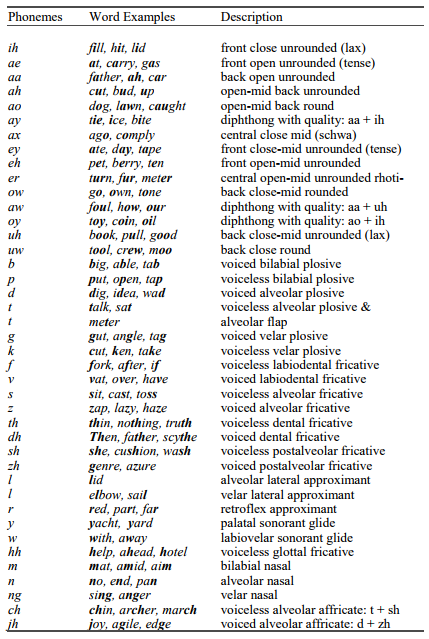
\includegraphics[width=0.35\textwidth]{phonemes}
	\caption{美式英语的音素和一般实现办法 \label{fig:exam-phonemes}}
\end{figure}

一般我们将音素分为两类:元音(Vowel)和辅音(Consonants)。
\begin{enumerate}
	\item Vowels:元音有两个特点,一是元音都是发声的声音(voiced sound),这意味着从声带(vocal chords)到口腔(mouth cavity)的气流是由声带的某种基频的震动(或者音高)产生的。二是舌头在生产过程中不会以任何方式形成气流收缩。每个元音发声的时候舌头、嘴唇和下巴的造型都不一样。这些不同的方式形成了不同的共振态,我们称之为共振峰。这些共振峰的共振态频率形成了不同的元音。
	\item Consonants:辅音是通过在口腔中或者空气中很明显的气流收缩形成的。有些辅音和元音一样是发声的,有些是不发声的。不发声的音素不会激活声带,因此也不存在基频或者音高。一些辅音音调成对出现,只有在有声或无声的情况下才有所不同,但在其他方面是相同的。比如说/b/和/p/这两个音素的发音方式是相同的,因为你的嘴唇、下巴还有舌头的姿势是一样的。但是/b/是发声的,/p/是不发声的。
\end{enumerate}

音素的另外一个重要特性是\textcolor{red}{其根据不同的上下文音素发音是会改变的}。我们称之为Phonetic Context。之所以会这样,是因为协同发音(coarticulation)。这些声音连续起来发音会改变其原有的特征。由协同发音产生的音素我们称为音素变体(allophones)。

所有当前的这些语音识别系统都使用了音素的语境相关的特性来建立处于不同phonetic context的音素模型。
% subsubsection phonetics (end)

\subsection{Words and Syntax} % (fold)
\label{sub:words_and_syntax}
Syllable 是一串声音,是个序列,由一个核心的音素,可能有初始音素和终止音素,这个核心音素一般是个元音或者一个音节辅音(syllablic consonant),是能够唱出来或者吼出来的声音。

举个例子,英文单词 "bottle" 包含两个 syllable 。第一个 syllable 有三个 phone ,在 Arpabet 音素描述代码里,是 "b aa t" 。这个 "aa" 就是核心音素,"b" 是发声的初始音素,"t" 是不发音的终止音素;第二个 syllable 是只包含一个 syllablic cosonant "l"。

一个 syllable 也可以组成一个词,其本身就是一个单独的音素,比如说,"Eye","uh",或者"eau"(医:水)。

语音识别里面,syllable 很少会考虑作为声学模型的建模单元,而词一般是变成音素来建模。

Syntax(句法规则)描述了给定词和定义了语法的规则下,句子的形成。而 Semantics(语义学)一般指代的是句子中的词或者短语是如何形成句意的。Syntax 和 Semantics 是 NLP 的重要组成部分,但是在语音识别里面,不起主要作用。
% subsection words_and_syntax (end)

\subsection{Measuring Performance} % (fold)
\label{sub:measuring_performance}
在语音识别系统的搭建和实验中,如何来衡量一个系统的好坏呢?由于语音识别是一个序列任务,跟图像当中的分类不一样,因此我们在衡量系统的性能时需要考虑到整个序列。

语音识别准确率衡量最常用的一个指标是词错误率(word error rate,WER)。一般识别出来的结果可能会产生三种错误:替换(substitution)、删除(delete)和插入(insert)。替换指的是一个词被识别成了另外一个词;删除指的是原本有词,但是没有识别出来;插入指的是原本没有词,多识别出来了词。WER 的计算方式如公式\ref{eqn:wer}。
\begin{align}
\label{eqn:wer}
	WER = \frac{N_{sub}+N_{ins}+N_{del}}{N_{ref}}
\end{align}
其中$N_{sub}$、$N_{ins}$和$N_{del}$分别是替换、插入和删除的数量,而$N_{ref}$是参考文本描述中词的个数。

WER的计算用的是通过计算实际输出描述和参考文本描述之间的\href{https://en.wikipedia.org/wiki/Edit_distance}{字符串编辑距离}得到的。编辑距离的实现通过动态规划算法。因为长文本的编辑距离可能不可靠,所以我们通过逐句的计算累积的错误,这些错误最终整合到一起来计算测试集的WER。编辑距离的原理见补充知识点中的\ref{sub:edit-distance}节。

表\ref{tab:wer}呈现了实际输出和参考文献之间的不同,以及对应的三种错误。
\begin{lstlisting}[language = python, numbers=left, 
				 numberstyle=\tiny,keywordstyle=\color{blue!70},
				 commentstyle=\color{red!50!green!50!blue!50},frame=shadowbox,
				 rulesepcolor=\color{red!20!green!20!blue!20},basicstyle=\ttfamily]
Ref: however a little later we had a comfortable chat
Hyp: how never a little later he had comfortable chat
\end{lstlisting}
\begin{table}[h]
 \centering
 \caption{WER计算公式中的三种错误实例演示}
	 \begin{tabular*}{1\textwidth}{@{\extracolsep{\fill}}ccc}
	 \toprule
		{\bf Reference} & {\bf Hypothesis} & {\bf Error} \\
	 \midrule
	 however      &        how  & Substitution \\ \hline
								&      never  &  Insertion   \\ \hline
				 a      &          a  &              \\ \hline
		little      &     little  &              \\ \hline
		later       &      later  &              \\ \hline
		we          &         he  & Substitution  \\ \hline
		had         &        had  &              \\ \hline
		a           &             &   Deletion   \\ \hline
	comfortable   & comfortable &              \\ \hline
			chat      &       chat  &              \\
	 \bottomrule
	 \end{tabular*}%
 \label{tab:wer}%
\end{table}%

在某些情况中,这三种错误的成本不对等,那么计算编辑距离的时候可以作相应的调整。

句错误率(Sentence Error Rate,SER)是另外一种衡量系统的标准,其计算方式是整句没有出现任何错误。SER 仅仅作为一个指标,来看下错误的句子占全部句子的比例。

% subsection measuring_performance (end)

\subsection{Significance Testing} % (fold)
\label{sub:significance_testing}
统计显著性检验(statistical significance testing)涉及测量两个实验(或算法)之间的差异在多大程度上归因于两个算法中的实际差异,或者仅仅是数据,实验设置或其他因素中的结果固有变异性。统计显著性是所有分类任务的基石,只是统计显著性检验的方法取决于任务的特性。大多数方法的核心是假设检验的概念中存在一个无效假设。问题在于你有多大的confidence能够说无效假设会被拒绝。

对于语音识别来说,比较两个实验或者算法最常用的方法是 Matched Pairs Sentence-Segment Word Error(MAPSSWE)检验,简称为 Matched Pairs Test\upcite{asr-sign}。

在这个方法中,测试集被分为几份,假设这些子测试集中任意一个的错误都与其他子测试集统计独立。这个假设和语音识别的实验很贴合,因为测试数据都是一句一句的经由识别器输出结果。给定了每一个句子的WER,就很容易构建一个matched pairs\upcite{Pallet1990Tools}。
% subsection significance_testing (end)

\subsection{Other Consideration} % (fold)
\label{sub:other_consideration}
除去准确率,对识别系统性能的影响还可能包括计算需求,处理速度或者延迟什么的。解码速度一般用实时因子(real-time factor,RTF)来衡量。RTF为1.0指的是系统处理10s的数据需要花10s的时间。

RTF高于1.0意味着系统要花更多的时间来解码,对于某些应用,也许是可以接受的,比如希望获得一个会议或者讲座的转写,相对于快速的得到转写结果,准确率可能更重要一些,因此多花一些时间也是可以接受的。

当RTF低于1.0,系统会在当前数据达到前就处理好了之前的数据。当不止一个系统在同一个机器上运行的时候,这个就比较有用了。在这种情况下,我们可以用多线程来并行处理多路音频流。此外RTF低于1.0意味着系统能够满足在线实时解码的音频流应用。比如说,当我们在处理一个手机上远程音频需求的时候,网络阻塞可能会使得服务器接收音频产生间隙和延迟。如果语音识别器能够以比实时更快的速度来处理,那么它就可以在数据达到之后迅速跟进,追上最新的音频进度,以速度来掩盖网络的延迟。

一般来说,语音识别系统能够在准确率和速度之间调整,但是这种调整也是有限的,不可能无限好或者无限快。对于一个给定的模型和测试集,speed-accuracy图有一条不可被突破的渐近线(asymptote),即便给予无限的算力。所以准确率是有个极限的,这个时候的错误率可以认为就是模型带来的错误。一旦根据模型搜索找到了最好的结果,进一步的处理也不会带来准确率上的提升。
% subsection other_consideration (end)

\subsection{The Fundamental Equation} % (fold)
\label{sub:the_fundamental_equation}
语音识别可以看作一个优化任务。特别地,给定一个观测序列$O=\{O_{1},...,O_{N}\}$,我们找寻的是最有可能的词序列$W=\{W_1,...,W_M\}$,也就是说我们要找到最大化后验概率$P(W|O)$的词序列,如公式\ref{eqn:fundamental-equation}。
\begin{align}
\label{eqn:fundamental-equation}
	\hat{W} = \arg\mathop{\max}_{W} P(W|O)
\end{align}
利用贝叶斯规则,我们得到公式\ref{eqn:fun-bayes}。
\begin{align}
\label{eqn:fun-bayes}
	P(W|O) = \frac{P(W)P(O|W)}{P(O)}
\end{align}

因为词序列并不依赖于观测序列的边缘概率分布$P(O)$,我们可以忽略这个部分,综合上述两个公式,我们得到公式\ref{eqn:fun-final}。
\begin{align}
\label{eqn:fun-final}
	\hat{W} = \arg\mathop{\max}_{W} P(W)P(O|W)
\end{align}

这就是语音识别的基本公式。语音识别问题就可以看作是在这个联合模型上的搜索。

公式中的$P(O|W)$叫做\textcolor{red}{声学模型(acoustic model)}。这个模型描述了在给定词序列$W$的条件下,声学观测$O$的分布。声学模型表征的是词序列是如何转换成声学实现的,进而转换成ASR系统的声学观测的。

公式中的$P(W)$叫做\textcolor{red}{语言模型(language model)},其只取决于词序列$W$。语言模型给每一个可能的词序列一个概率值。它是由日常使用的一些词序列训练成的。一个训练好的英语语言模型会给"I like turtles"高的概率值,给"Turtles sing table"低的概率值。语言模型促使着词序列的搜索沿着训练数据中的模式开展。语言模型也可以在一些纯文本的应用中见到,比如浏览器的自动补全等。

由于诸多原因,构建一个语音识别系统比这个简单地公式所能呈现的要复杂的多得多。
% subsection the_fundamental_equation (end)
\subsection{Lab 1: Create a speech recognition scoring program} % (fold)
\label{sub:lab-1}
本模块有一个实验作业,标题为"Create a speech recognition scoring program"。

{\bf Required files:}
\begin{itemize}
	\item \textcolor{blue}{wer.py}
	\item \textcolor{blue}{M1\_score.py}
\end{itemize}}

{\bf Instructions:}

In this lab, you will write a program in Python to compute the word error rate (WER) and sentence error rate (SER) for a test corpus. A set of hypothesized transcriptions from a speech recognition system and a set of reference transcriptions with the correct word sequences will be provided for you.

This lab assumes the transcriptions are in a format called the "trn" format, created by NIST. The format is as follows. The transcription is output on a single line followed by a single space and then the root name of the file, without any extension, in parentheses. For example, the audio file "tongue\_twister.wav" would have a transcription

sally sells seashells by the seashore (tongue\_twister)

Notice that the transcription does not have any punctuation or capitalization, nor any other formatting (e.g. converting "doctor" to "dr.", or "eight" to "8"). This formatting is called "Inverse Text Normalization" and is not part of this course.

The python code \textcolor{blue}{M1\_Score.py} and \textcolor{blue}{wer.py} contain the scaffolding for the first lab. A main function parses the command line arguments and string\_edit\_distance() computes the string edit distance between two strings.

Add code to read the trn files for the hypothesis and reference transcriptions, to compute the edit distance on each, and to aggregate the error counts. Your code should report:
\begin{itemize}
	\item Total number of reference sentences in the test set
	\item Number of sentences with an error
	\item Sentence error rate as a percentage
	\item Total number of reference words
	\item Total number of word errors
	\item Total number of word substitutions, insertions, and deletions
	\item The percentage of total errors (WER) and percentage of substitutions, insertions, and deletions
\end{itemize}

The specific format for outputting this information is up to you. Note that you should not assume that the order of sentences in the reference and hypothesis trn files is consistent. You should use the utterance name as the key between the two transcriptions.

When you believe your code is working, use it to process hyp.trn and ref.trn in the misc directory, and compare your answers to the solution.

{\bf Solutions:}

我们将课程提供的代码补充完整,加上对应的代码注释和结果展示。首先说下测试文本的格式。测试文本有两个
\begin{itemize}
	\item {\bf hyp.trn}:模型输出结果;
	\item {\bf ref.trn}:参考文本。
\end{itemize}

hyp.trn的内容如下:
\begin{lstlisting}[language = python, numbers=left, 
				 numberstyle=\tiny,keywordstyle=\color{blue!70},
				 commentstyle=\color{red!50!green!50!blue!50},frame=shadowbox,
				 rulesepcolor=\color{red!20!green!20!blue!20},basicstyle=\ttfamily]
apple coconut date eggplant elephant fig (0000-000000-0000)
one tiger three flamingo five six (0000-000000-0001)
delaware cat georgia dog mouse massachusetts  (0000-00000-0002)
\end{lstlisting}

ref.trn的内容如下:
\begin{lstlisting}[language = python, numbers=left, 
				 numberstyle=\tiny,keywordstyle=\color{blue!70},
				 commentstyle=\color{red!50!green!50!blue!50},frame=shadowbox,
				 rulesepcolor=\color{red!20!green!20!blue!20},basicstyle=\ttfamily]
apple banana coconut date eggplant fig (0000-000000-0000)
one two three four five six (0000-000000-0001)
delaware pennsylvania new_jersey georgia connecticut massachusetts  (0000-00000-0002)
\end{lstlisting}

可以很明显的看到,hyp和ref是一一对应的,格式相同,都是trn文件,其内部都是"text (token)"的形式。

本节的代码逻辑是构建一个函数{\bf string\_edit\_distance},其接受ref和hyp两个变量,返回的是一个tuple,依次为token、edits、deletions、insertions和substitutions。该函数存储于{\bf wer.py}中,以供代码{\bf M1\_score.py}调用。

我们先来看{\bf wer.py},理解了函数{\bf string\_edit\_distance}自然就会调用了。代码和注释如下:
\begin{lstlisting}[language = python, numbers=left, 
				 numberstyle=\tiny,keywordstyle=\color{blue!70},
				 commentstyle=\color{red!50!green!50!blue!50},frame=shadowbox,
				 rulesepcolor=\color{red!20!green!20!blue!20},basicstyle=\ttfamily]
import numpy as np


def string_edit_distance(ref=None, hyp=None):

		if ref is None or hyp is None:
				RuntimeError("ref and hyp are required, cannot be None")

		x = ref
		y = hyp
		tokens = len(x)
		if (len(hyp)==0):
				return (tokens, tokens, tokens, 0, 0)

		# p[ix,iy] consumed ix tokens from x, iy tokens from y
		p = np.PINF * np.ones((len(x) + 1, len(y) + 1)) # track total errors
		e = np.zeros((len(x)+1, len(y) + 1, 3), dtype=np.int) # track deletions, insertions, substitutions
		p[0] = 0
		for ix in range(len(x) + 1):
				for iy in range(len(y) + 1):
						cst = np.PINF*np.ones([3])
						s = 0
						if ix > 0:
								cst[0] = p[ix - 1, iy] + 1 # deletion cost
						if iy > 0:
								cst[1] = p[ix, iy - 1] + 1 # insertion cost
						if ix > 0 and iy > 0:
								s = (1 if x[ix - 1] != y[iy -1] else 0)
								cst[2] = p[ix - 1, iy - 1] + s # substitution cost
						if ix > 0 or iy > 0:
								idx = np.argmin(cst) # if tied, one that occurs first wins
								p[ix, iy] = cst[idx]

								if (idx==0): # deletion
										e[ix, iy, :] = e[ix - 1, iy, :]
										e[ix, iy, 0] += 1
								elif (idx==1): # insertion
										e[ix, iy, :] = e[ix, iy - 1, :]
										e[ix, iy, 1] += 1
								elif (idx==2): # substitution
										e[ix, iy, :] = e[ix - 1, iy - 1, :]
										e[ix, iy, 2] += s

		edits = int(p[-1,-1])
		deletions, insertions, substitutions = e[-1, -1, :]
		return (tokens, edits, deletions, insertions, substitutions)
\end{lstlisting}
% subsection lab (end)

%------------------------------------------------------------------------------
%                                Speech Signal Processing
%------------------------------------------------------------------------------
\section{Speech Signal Processing}
\subsection{Introduction} % (fold)
\label{sub:introduction}
通过空气传播的音频波形通过麦克风的捕捉,将这些压力波转换成可捕捉的电信号活动。对这些电信号活动进行采样,这样就得到了一系列采样波形,我们用这些波形来描述信号。音乐信号一般采样率为 44100 Hz,即一秒钟会有44100个采样点。根据奈奎斯特定理(Nyquist theorem),只有频率低于22050 Hz的音频才可以被捕捉到。如果信号的高频部分比较少,最高频率为8000Hz的话,采样率一般就是16000Hz。传统的电话和大部分的手机带限是3400 Hz,所以8000 Hz的采样率就足够了。所以电话语音的采样率一般就是 8000Hz。

一个典型的音频波形图如\ref{fig:wavform}(左),其说的句子是"speech recognition is cool stuff"。
\begin{figure}[!ht]
	\centering
	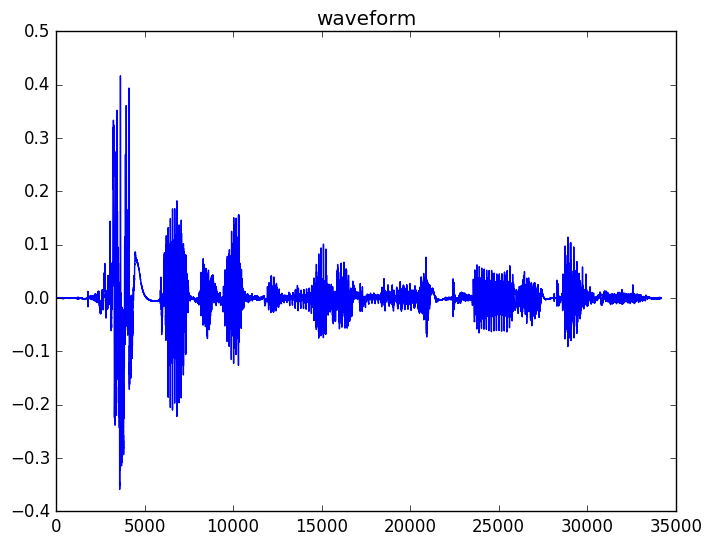
\includegraphics[width=0.45\textwidth]{waveform}
	\hspace{1cm}
	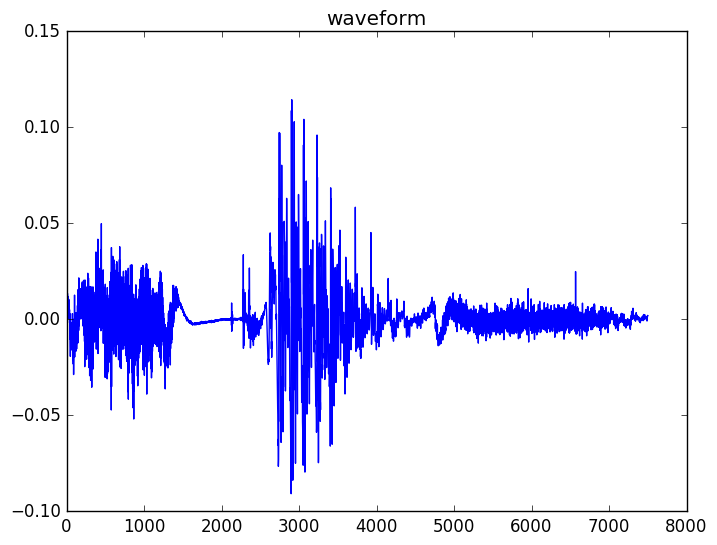
\includegraphics[width=0.45\textwidth]{stuff}
	\hspace{1cm}
	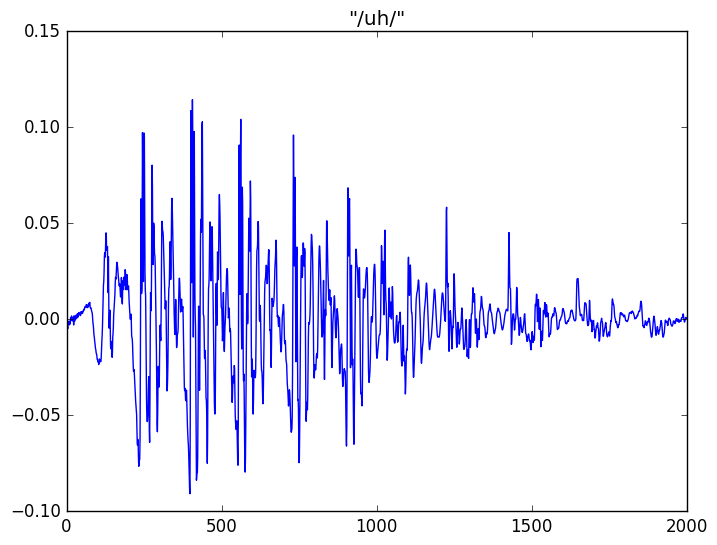
\includegraphics[width=0.45\textwidth]{uh}
	\caption{完整音频波形图与部分波形图}
\label{fig:wavform}
\end{figure}

回忆上一节中讨论的发声音素和不发声音素,我们来瞅一下最后一个单词 "stuff" 的波形图,如图\ref{fig:wavform}(右)。从图上我们看到,这个单词的发音有三个不同的部分,初始不发声语音"st",中间发声语音"uh",终止不发声语音"f"。不发声的语音部分看上去像噪音,具有随机性。而发声部分的语音由于声带的振动而具有周期性。

在拉近一点,我们看看发声的这个元音"/uh/",如图\ref{fig:wavform}(下)可以更明显的看到这个元音的周期性。

从这些波形图中,我们可以看到波形的特征形成有两方面的因素:(1)声带的应激反应(excitation)趋势着空气从声道和嘴巴流出;(2)发出某种特定声音时,声道本身的形状。

举例来说,图\ref{fig:wavform}(右)中"st"和"f"看上去都像噪声,但是他们的形状却不相同,就是因为他们是不一样的声音。而"uh"的声音更具周期性,因为发声的应激反应,其由于发声的时候声道的作用有独特的形状。所以对于同一个说话人来说,不同的元音可能会有着相近的周期,但是波形的整体形状是不一样的,就因为这些波形都是由相同的声带产生的,但是发不同的声音声道是不一样的。

在信号处理中,一般用源滤波器模型(source-filter model)来对这个语音产生的过程进行建模。声源是由通过声道的声带产生的激励信号,我们将其建模成为时变线性滤波器。源滤波器在语音识别中有很多应用,比如语义分析和编码。而且有很多种办法来评估源信号和滤波器的参数,比如很有名的线性预测编码(Linear Predictive Coding,LPC)。

对于语音识别来说,音素分类在很大程度上取决于声道的形状,也就是说取决于源滤波器模型的滤波器部分。激励信号或者原信号大都被忽略或者舍弃了。所以语音识别的特征提取过程一般设计成捕捉话语过程的时变滤波器形状。
% subsection introduction (end)

\subsection{Feature Extraction} % (fold)
\label{sub:feature_extraction}
从波形图中,很明显语音是非平稳信号(non-stationary signal),这就意味着语音信号的统计特性会随着时间变化而变化。所以为了分析语音信号,我们需要将信号分成一个又一个 chunk(也成为窗或者帧),这些chunk短到可以认为它们是平稳信号。这样我们就可以去分析一系列短时的有重叠的语音帧。在语音识别中,我们一般选窗长为 25ms,窗移位 10ms,也就是说一秒钟会被分成100帧。

因为我们是从一个长音频提取的chunk,所以对于每一个chunk的边缘,我们要进行一些处理。一般对每一帧数据加个窗函数,常用的是汉明窗(Hamming Windows),当然也有用其他窗函数的。定义$m$为某一帧的索引,$n$为采样点的索引,$L$是这一帧采样点的个数,$N$是采样中的偏移量。那么从原始信号中提取出来的每一帧计算公式见\ref{eqn:frame-window}。
\begin{align}
\label{eqn:frame-window}
	x_{m}[n]=w[n] x[m N+n], n=0,1, \ldots, L-1
\end{align}
其中$w[n]$是窗函数。

然后我们利用离散傅里叶变换将每一帧的数据转换到频域,如公式\ref{eqn:fft}。所有现代软件中都可以有效的计算快速傅里叶变换。
\begin{align}
\label{eqn:fft}
	X_{m}[k]=\sum_{n=0}^{N-1} x_{m}[n] e^{-j 2 \pi k n N}
\end{align}

傅里叶表征$X_{M} [k]$是一个很复杂的数,因为它包含了每一帧和每一个频率的频谱幅值(绝对幅值)和相位信息。为了提取特征,我们去掉了相位信息,只考虑幅值 $|X_{m}[k]|$。

频谱图描述了对语音信号进行FFT操作得到的log幅值(或者log-power),如图\ref{fig:log-compare}(右)。横轴是帧索引(单位为10ms),纵轴是频率,其范围是0Hz到采样率的一般,也就是对应的Nyquist频率。图中呈现的是"speech recognition is cool stuff"。在频谱图中,黄色和红色区域表示该区域能量高。
% subsection feature_extraction (end)

\subsection{Mel Filtering} % (fold)
\label{sub:mel_filtering}
从频谱图中可以看出高频的高能量区域大致对应着不发声的辅音,低频的高能量区域大致对应着发声的元音。频谱图中,发声区域的水平线(horizonal lines)呈现的是语音的谐波结构(harmonic structure)。

由于发声区域的谐波结构和不发声区域的随机噪声,频谱中存在着变数(variability)。为了移除这些变数,我们对幅度谱(magnitude spectrum)进行频谱光滑操作。受听觉系统处理语音信号的启发,我们对频谱图进行滤波器组操作(filterbank),该滤波器组对频率轴进行了 approximately logarithmic scale。也就是说随着频率的升高,滤波器也会变得更宽间隔更大。最常用于特征提取的filterbank是 {\bf mel filterbank}。一个 mel filterbank 包含40个滤波器,如图\ref{fig:mel-fbank}。每一个滤波器会对不同频率区间的能量谱求平均。
\begin{figure}[htbp]
	\centering
	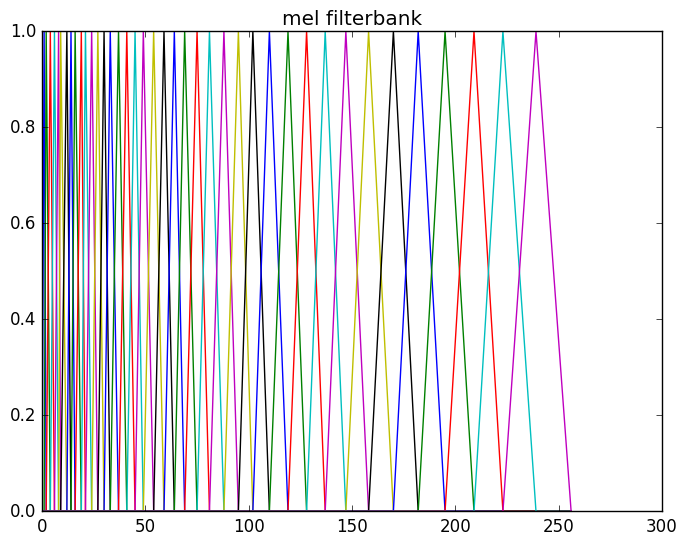
\includegraphics[width=0.45\textwidth]{mel-fbank}
	\caption{mel filterbank \label{fig:mel-fbank}}
\end{figure}

mel filterbank图在左边的滤波器很密集,在右边的滤波器间隔就比较远了。这是符合人耳听觉系统的,因为人耳对低频的信号更加敏感,对高频的信号不太敏感,所以低频的信息是更重要的,那么就需要多一些滤波器,从而提取更多有效特征。

P维的 mel filterbank的系数计算公式如\ref{eqn:mel-fbank}。一个 mel filterbank一般会计算出40个系数,虽然现代系统有的会多一些或者少一些。平滑过多,系数就少一些,反之则反之。
\begin{align}
\label{eqn:mel-fbank}
	X_{\mathrm{mel}}[p]=\sum_{k} M[p, k]\left|X_{m}[k]\right|, \quad p=0,1, \ldots, P-1
\end{align}

% subsection mel_filtering (end)

\subsection{Log Compression} % (fold)
\label{sub:log_compression}
特征提取的最后一步是对经过滤波器组得到的系数进行对数压缩。这个操作有助于压缩信号的动态范围,还能模拟听觉系统对声音的非线性压缩效果。我们把对数压缩后的输出称为 "filterbank" 系数。

将提取的特征以频谱图式的方式呈现出来之后,如图\ref{fig:log-compare}(左),与原始信号频谱图(右)进行比较,我们可以看出沿着频率轴的Fbank系数要平滑得多,这是因为高频噪声和pitch/谐波结构都被移除了。
\begin{figure}[!ht]
	\centering
	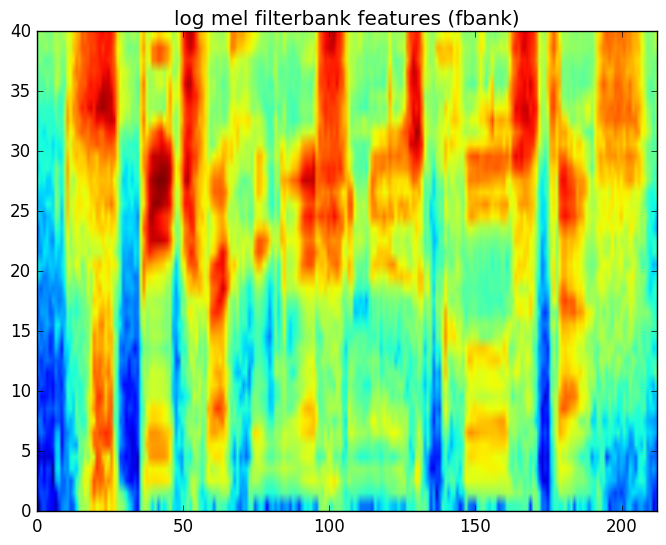
\includegraphics[width=0.45\textwidth]{figure/log-mel-fbank}
	\hspace{1cm}
	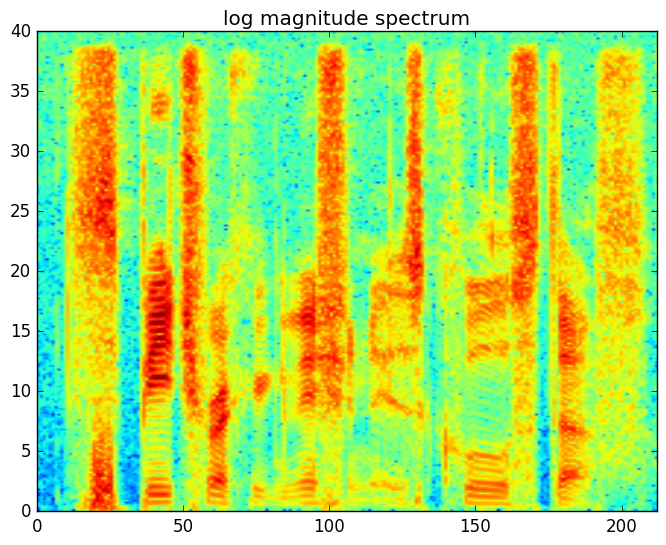
\includegraphics[width=0.45\textwidth]{figure/log-power}
	\caption{提取Fbank特征(左)与原始信号的频谱图(右)}
\label{fig:log-compare}
\end{figure}
% subsection log_compression (end)

除了上面的这些操作,在提取特征的过程中可能还会有一些其他的操作。其中有:
\begin{enumerate}
	\item Dithering(抖动):在原始音频信号中加入一个很小的噪声,为了防止在提取特征的时候出现数学问题,尤其是出现$\log0$;
	\item DC-removal(直流常数移除):在提取特征之前,去除音频中的常数偏置;
	\item Pre-emphasis(预加重):在提取特征之前用一个高通滤波器处理信号,因为发声的语音部分低频能量比不发声的语音部分高频能量要大得多,用一个高通滤波器来抵消下这个问题。实际操作的时候就是用了一个简单地线性滤波器,见公式\ref{eqn:pre-emp},其中$\alpha=0.97$。
		\begin{align}
		\label{eqn:pre-emp}
		y[n]=x[n]-\alpha x[n-1]
		\end{align}
	\item DCT(离散余弦变换):Fbank系数是强相关的,为了减弱这种相关性,将上述步骤提取出来的Fbank特征值再经过DCT。经过DCT之后的特征,一般取前13个,余下的由于所含信息不足舍弃了。DCT公式如\ref{eqn:dct}。
		\begin{align}
		\label{eqn:dct}
		d_t =\frac{\sum_{n=1}^{N}n(c_{t+n}-c_{t-n})}{2\sum_{n=1}^{N}n^2}
		\end{align}
\end{enumerate}}

\subsection{Feature Normalization} % (fold)
\label{sub:feature_normalization}
通信信道可能会对捕获的语音信号引入一些偏差(恒定滤波)。比如说,麦克风的频率响应不平稳,此外,即使相同语音的基础信号,其信号增益的变化也可能导致计算的滤波器组系数的差异。这些信道的影响可以用时域上的卷积进行建模,等价于频域表征的信号进行点乘(elementwise multiplication)。

因此信道的影响可以用恒定滤波来建模(constant filter),如公式\ref{eqn:model-channel}。
\begin{align}
\label{eqn:model-channel}
X_{t, \mathrm{obs}}[k]=H[k] X_{t}[k]
\end{align}
其观测幅度为:
\begin{align}
\label{eqn:ob-mag}
\left|X_{t, \mathrm{obs}}[k]\right|=|H[k]|\left|X_{t}[k]\right|
\end{align}

如果我们对公式\ref{eqn:ob-mag}两边取对数,并计算句子中所有帧的均值,则我们有公式\ref{eqn:log-mean}。
\begin{align}
\begin{split}
\label{eqn:log-mean}
\mu_{\mathrm{obs}}
		&=\frac{1}{T} \sum_{t} \log \left(\left|X_{t, \mathrm{obs}}[k]\right|\right) \\
		&=\frac{1}{T} \sum_{t} \log \left(|H[k]|\left|X_{t}[k]\right|\right) \\
		&=\frac{1}{T} \sum_{t} \log (|H[k]|)+\frac{1}{T} \sum_{t} \log \left(\left|X_{t}[k]\right|\right)\\
\end{split}
\end{align}

假设滤波器在时间轴上是常数,且语音信号的对数幅值均值为0,那么公式\ref{eqn:log-mean}可以简化为\ref{eqn:log-mean-simple}。
\begin{align}
\label{eqn:log-mean-simple}
	\mu_{t t o b s}=\log (|H[k]|)
\end{align}

以上,如果我们计算出句子的对数幅值的均值,并且对句子中的每一帧都减去这个均值,这样我们就可以除去信号中所有的恒定信道效应。

为了简便,我们直接对取了$\log$之后fbank特征进行归一化(normalization)。为了对比一系列操作的结构,图\ref{fig:fbank-normalization}展现了原始信号的频谱图(左)、fbank特征的频谱图(右)和对fbank特征归一化后的频谱图(下)。
\begin{figure}[!ht]
	\centering
	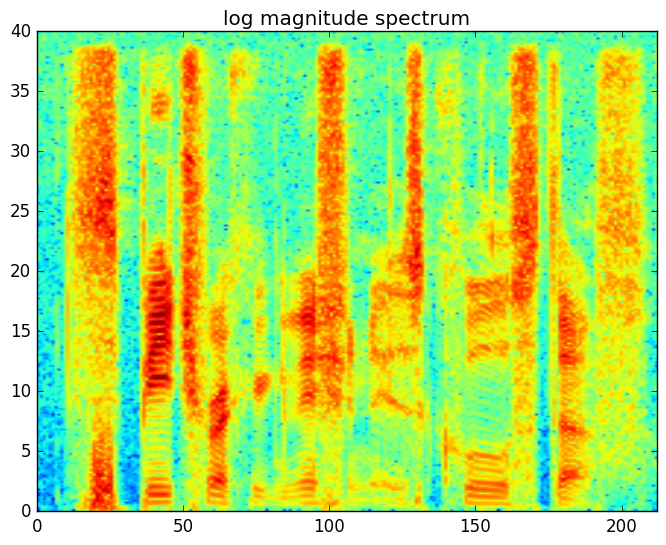
\includegraphics[width=0.40\textwidth]{figure/log-power}
	\hspace{0.5cm}
	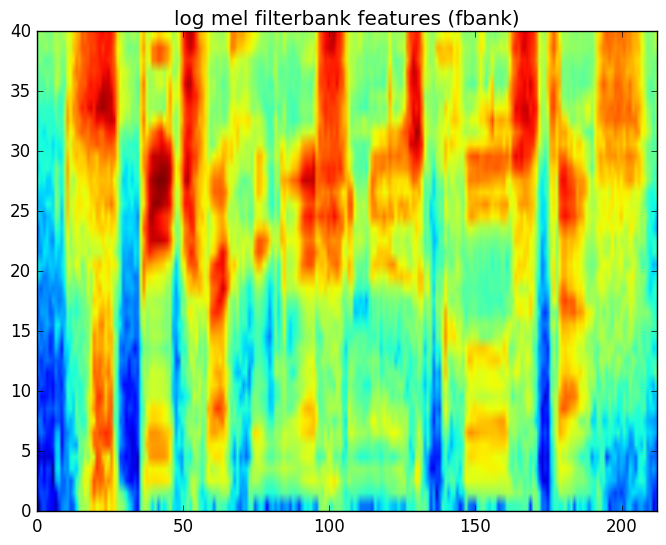
\includegraphics[width=0.40\textwidth]{figure/log-mel-fbank}
	\hspace{0.5cm}
	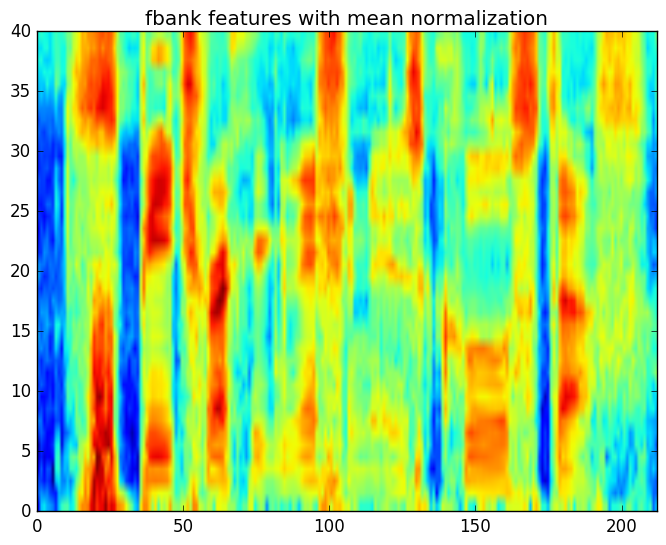
\includegraphics[width=0.40\textwidth]{figure/log-mel-fbank-norm}
	\caption{原始信号的频谱图(左)、提取Fbank特征(右)和归一化后的Fbank特征(下)}
\label{fig:fbank-normalization}
\end{figure}
% subsection feature_normalization (end)
\subsection{Summary}
为了从语音信号中提取语音识别所需的特征,我们希望提取到与声道形状有关的时变频谱信息,其由源滤波器模型中的一个滤波器建模,计算语句中的特征步骤如下:
\begin{enumerate}
	\item 预处理信号,包括预加重和dithering;
	\item 将信号切割成有重叠部分的帧,一般帧长为 25ms,帧移为 10ms;
	\item 对于每一帧:
			\begin{itemize}
				\item 用汉明窗处理信号;
				\item 使用FFT进行傅里叶变换;
				\item 计算频谱的幅值;
				\item 应用 mel filterbank;
				\item 进行对数操作;
			\end{itemize}
	\item 如果需要进行信道补偿,则对每一帧的fbank系数进行均值归一化。
\end{enumerate}

\subsection{Lab 2: Feature extraction for speech recognition} % (fold)
\label{sub:lab_2}
本模块有一个实验作业,标题为"Feature extraction for speech recognition"。

{\bf Required files:}
\begin{itemize}
	\item \textcolor{blue}{M2\_Wav2Feat\_Single.py}
	\item \textcolor{blue}{M2\_Wav2Feat\_Batch.py}
	\item \textcolor{blue}{speech\_sigproc.py}
	\item \textcolor{blue}{htk\_featio.py}
\end{itemize}}

{\bf Instructions:}

In this lab, you will write the core functions necessary to perform feature extraction on audio waveforms. Your program will convert an audio file to a sequence of log mel frequency filterbank ("FBANK") coefficients.

The basic steps in features extraction are
\begin{enumerate}
	\item Pre-emphasis of the waveform
	\item Dividing the signal into overlapping segments or frames
	\item For each frame of audio:
		\begin{itemize}
			\item Windowing the frame
			\item Computing the magnitude spectrum of the frame
			\item Applying the mel filterbank to the spectrum to create mel filterbank coefficients
			\item Applying a logarithm operation to the mel filterbank coefficient
		\end{itemize}
\end{enumerate}
In the lab, you will be supplied with python file called {\bf speech\_sigproc.py}. This file contains a partially completed python class called {\bf FrontEnd} that performs feature extraction, using methods that perform the steps listed above. The methods for dividing the signal into frames (step 2) will be provided for you, as will the code for generating the coefficients of the mel filterbank that is used in step 3c. You are responsible for filling in the code in all the remaining methods.

There are two top-level python scripts that call this class. The first is called {\bf M2\_Wav2Feat\_Single.py}. This function reads a single pre-specified audio file, computes the features, and writes them to a feature file in HTK format.

In the first part of this lab, you are to complete the missing code in the {\bf FrontEnd} class and then modify {\bf M2\_Wav2Feat\_Single.py} to plot the following items:
\begin{enumerate}
	\item Waveform
	\item Mel frequency filterbank
	\item Log mel filterbank coefficients
\end{enumerate}

You can compare the figures to the figures below. Once the code is verified to be working, the feature extraction program should be used to create feature vector files for the training, development, and test sets. This will be done using {\bf M2\_Wav2Feat\_Batch.py}. This program takes a command line argument {\bf –-set} (or {\bf -s} ) which takes as an argument either {\bf train}, {\bf dev}, or {\bf test}. For example

{\bf \$ python M2\_Wav2Feat\_Batch.py –set train}

This program will use the code you write in the {\bf FrontEnd} class to compute feature extraction for all the files in the LibriSpeech corpus. You need to call this program 3 times, once each for train, dev, and test sets.

When the training set features are computed ({\bf –set train}) the code will also generate the global mean and precision (inverse standard deviation) of the features in the training set. These quantities will be stored in two ASCII files in the {\bf am} direction for use by CNTK during acoustic model training in the next module.

Here are the outputs you should get from plotting:
\begin{figure}[!ht]
	\centering
	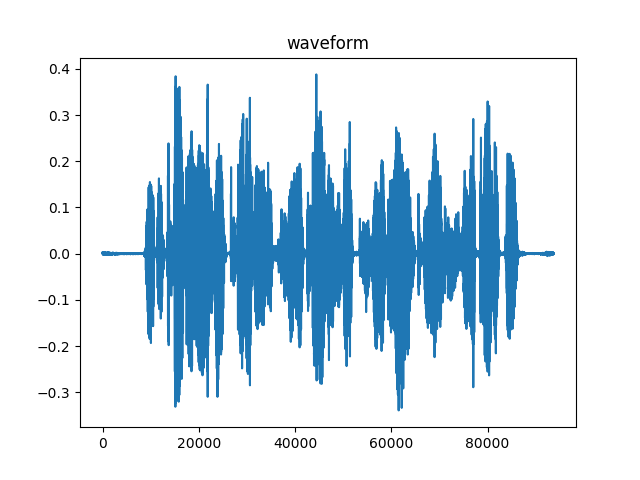
\includegraphics[width=0.30\textwidth]{figure/lab2-1}
	\hspace{0.5cm}
	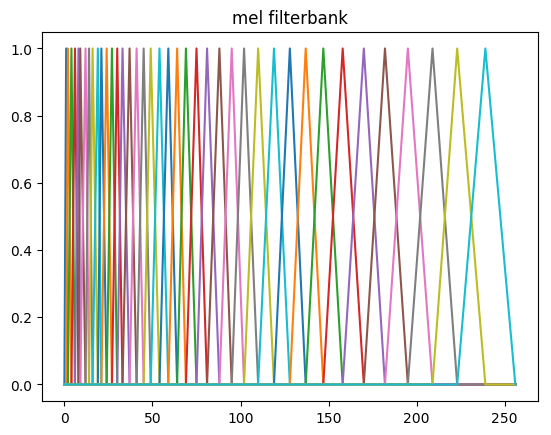
\includegraphics[width=0.30\textwidth]{figure/lab2-2}
	\hspace{0.5cm}
	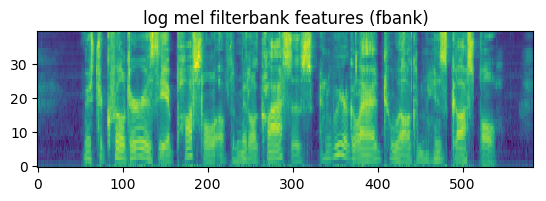
\includegraphics[width=0.30\textwidth]{figure/lab2-3}
	\caption{Lab 2的期望输出}
\label{fig:expect-output}
\end{figure}
% subsection lab_2 (end)

%------------------------------------------------------------------------------
%                                Acoustic Model
%------------------------------------------------------------------------------
\section{Acoustic Modeling}
\subsection{Introduction} 
本节讨论的是语音识别器中的声学模型。声学模型是一个混合模型,通过DNN得到逐帧的预测标签,再通过HMM将这些预测的音素转换成序列预测。HMM常用于对离散时间序列事件的建模。HMM的基本概念可以追溯到数十年前,而且HMM有很多应用。

\subsection{Markov Chains} 
了解一点马尔科夫链(Markov Chains)对学习HMM大有帮助。马尔科夫链是一种对随机过程进行建模的方法。在马尔科夫链中,用一系列状态(states)来对离散时间进行建模。状态之间的运动由随机过程控制。

举例说明,在一个天气预测的应用中,状态为 "{\bf S}unny"、"{\bf P}artly Cloud"、"{\bf C}loudy"、和"{\bf R}aining"。我们考虑某个连续五天的特定天气概率,比如$P(p,p,c,r,s)$,我们可以使用贝叶斯规则将这个联合概率分布打散成一系列条件概率的乘积,如公式\ref{eqn:markov1}。
\begin{align}
\label{eqn:markov1}
	p(X_1, X_2, X_3, X_4, X_5)=p(X_5 | X_4, X_3, X_2, X_1) p(X_4 | X_3, X_2, X_1) p(X_3 | X_2, X_1) p(X_2 | X_1) p(X_1)
\end{align}

假设天气模型满足一阶马尔科夫假设,即满足公式\ref{eqn:first-order}。
\begin{align}
\label{eqn:first-order}
	p(X_i |X_1, ..., X_{i-1})=p(X_i | X_{i-1})
\end{align}

那么连续五天天气的联合概率分布可以简化为公式\ref{eqn:markov2}。
\begin{align}
\label{eqn:markov2}
\begin{split}
	p(X_1, X_2, X_3, X_4, X_5)
			&= p(X_5 | X_4) p(X_4 | X_3) p(X_3 | X_2) p(X_2 | X_1) p(X_1) \\
			&= p(X_1)\prod_{i=2}^{5}p(x_i|x_{i-1})
\end{split}
\end{align}

一个马尔科夫链的核心元素有\textcolor{red}{状态的定义}(此处为天气预测)和\textcolor{red}{转移概率$p(X_i|X_{i-1})$},转移概率描述的是从一个状态移动到另一个状态的概率值(也包括转移到自身状态)。

比如说,天气预报的一个完整的(大体完整的)马尔科夫链可以用图\ref{fig:markov-weather}来表示。
\begin{figure}[htbp]
	\centering
	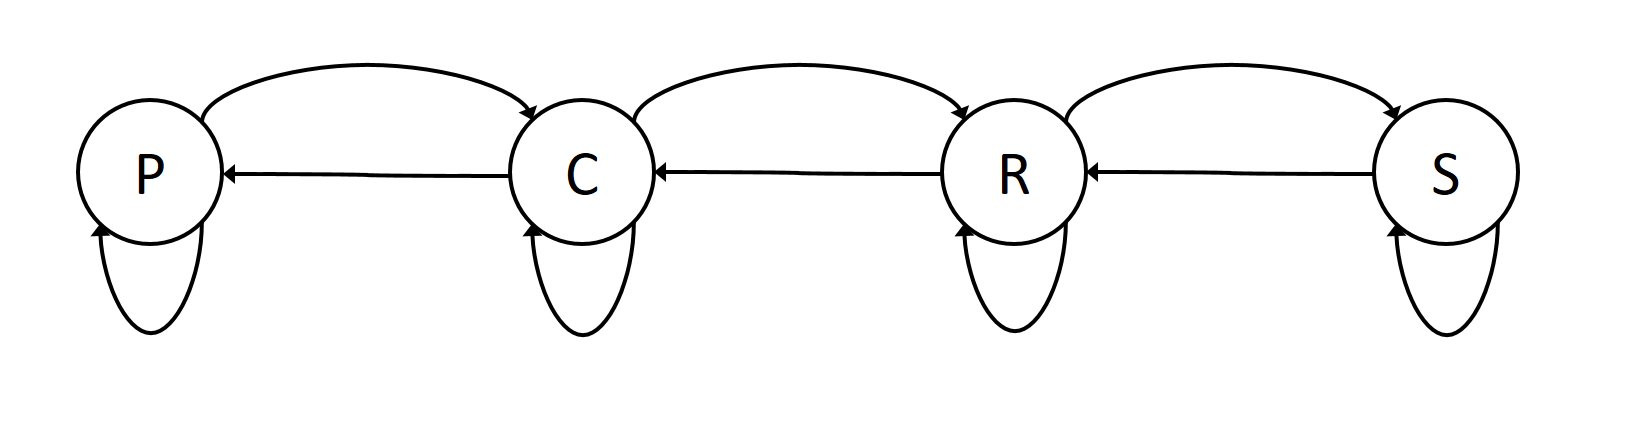
\includegraphics[width=0.45\textwidth]{markov-weather}
	\caption{天气预报模型的马尔科夫链\label{fig:markov-weather}}
\end{figure}

需要注意的是除了上面说的转移概率$p(X_i|X_{i-1})$,我们还需要知道这个序列的第一个元素,即第一天的某种天气的概率值$p(X_1)$。

所以除了状态清单和状态转移概率,我们还需要知道从马尔科夫链每一个状态开始的初始概率值。假设先验概率(每个状态的初始概率值)如公式\ref{eqn:markov-prior}。
\begin{align}
\label{eqn:markov-prior}
\begin{split}
	p(p) &= \pi_{p} \\
	p(c) &= \pi_{c} \\
	p(s) &= \pi_{s} \\
	p(r) &= \pi_{r}
\end{split}
\end{align}

现在我们回到这个例子,公式\ref{eqn:markov-weather-solu}说明了如何求$P(p,p,c,r,s)$。
\begin{align}
\label{eqn:markov-weather-solu}
\begin{split}
	p(p,p,c,r,s) &= p(s|p,p,c,r)p(r|p,p,c)p(c|p,p)p(p|p)p(p) \\
							 &= p(s|r) p(r|c) p(c|p) p(p|p) p(p)
\end{split}
\end{align}

上述Markov Models也可以称为可观测的马尔科夫模型(observable markov models)。因为当某个时刻所处状态已知,其输出是显性可见的,比如说今天会下雨。而HMM中的每个状态的输出并不是确定性事件或者确定性观察,而是事件或者观察的概率分布。这就使得HMM是双随机的(double stochastic):状态之间的转移是随机的,状态的观测值也是随机的。

同样以天气举例子,我们可以将天气系统的Markov model转变成HMM,将原先的状态 "{\bf S}unny"、"{\bf P}artly Cloud"、"{\bf C}loudy"、和"{\bf R}aining"替换成"Hot"、"Chilly"、"Cold"和"Stormy",这些状态以不同的概率值对应着不同的天气,如图\ref{fig:hmm-we},当状态为"Hot"的时候,观测值有$0.9$的概率为"Sunny",有$0.1$的概率为"Partly Cloudy"。
\begin{figure}[htbp]
	\centering
	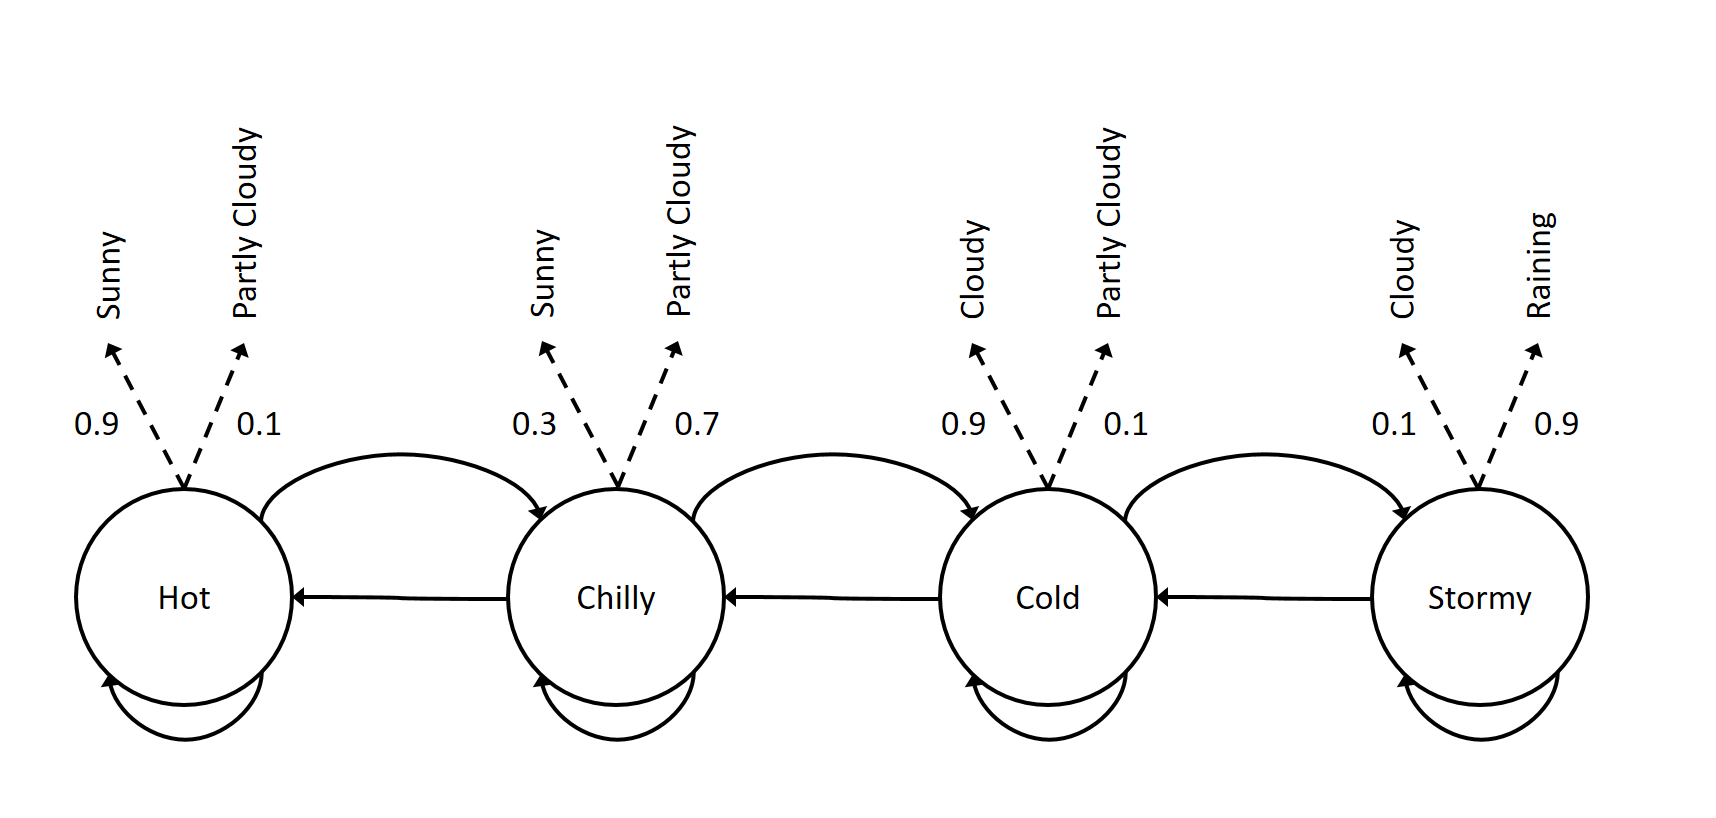
\includegraphics[width=0.45\textwidth]{hmm-weather}
	\caption{天气预报模型的隐马尔科夫模型\label{fig:hmm-we}}
\end{figure}

因此一个包含了$N$个状态的HMM模型,其参数为:
\begin{itemize}
	\item 转移矩阵$A$,其元素为$a_{ij}$,表征了从一个状态跳转到下一个状态的转移概率;
	\item 发射矩阵$B$,其元素为$b_i{x}$,表征了状态$i$的观测值为$x$的概率值,其中$i=1,2,...,N$;
	\item 初始化状态的先验概率,即初始状态为某个状态的概率值,$\pi=\{\pi_{1}, \pi{2},...,\pi_{N}\}$。
\end{itemize}

我们将这些参数记成$\Phi=\{A,B,\pi\}$。

HMM有三个基本问题,每一个问题都有着很牛逼的解决办法,此处仅做一个简单介绍,详细的过程参考\ref{sub:hmm}节。

{\bf The Evaluation Problem}

\textcolor{blue}{给定一个模型和观测序列,这些观测序列由这个模型生成的概率有多大?}

这个问题可以通过将所有可能的状态序列的概率加起来求得,这些状态序列都可以产生观测序列,通过转移概率和发射概率就可以求得。但是直接这么干是不划算的,因为其时间复杂度为$O(N^{T})$,其中$T$为观测序列的长度,$N$为所有可能的观测序列。

前向算法是一种动态规划算法,相比较而言要有效得多。前向算法是在每个时间步都处理下子序列的前向概率。其在每个时间步都会存储$N$个值,时间复杂度为$O(N^{2}T)$。

{\bf The Decoding Problem}

\textcolor{blue}{给定一个模型和观测序列,最有可能产生这个观测序列的状态序列是什么?}

这个问题可以用Viterbi算法解决,Viterbi算法被广泛的应用于语音识别的解码上,后续我们会介绍其是如何应用于语音识别以及如何将Viterbi算法并入训练准则之中。

{\bf The Training Problem}

\textcolor{blue}{给定一个模型和观测序列,如何去估计模型的参数$\Phi$?}

这个问题可以用Baum-Welch算法来解决,这个算法中就包含了前后向算法。本处的前向算法计算了$t$时刻处于状态$i$的所有可能的子序列的前向概率,后向算法计算了$t$时刻处于状态$i$为出发点直到$T$的所有可能的子序列的后向概率,此时时间步的初始值为$t+1$,因此将前后向算法合并起来就是整个$T$时间步,所有在$t$时刻处于状态$i$的路径概率之和。

我们知道了每一个时刻各个状态的后验概率之后,Baum-Welch算法将这些后验概率作为隐藏状态序列的直接观测值,并且更新模型的参数来优化目标函数。

\subsection{Hidden Markov Models for Speech Recognition} 
在语音识别中HMM用于对声学观测(声学特征向量)建模,其建模单元为子词,比如说音素。

典型的做法是一个音素对应三个HMM的状态,用于对这个音素的开始、中间和结尾建模,每个状态有个自转移概率和转移到下一个状态的概率值,如图\ref{fig:hmm-uh}。
\begin{figure}[htbp]
	\centering
	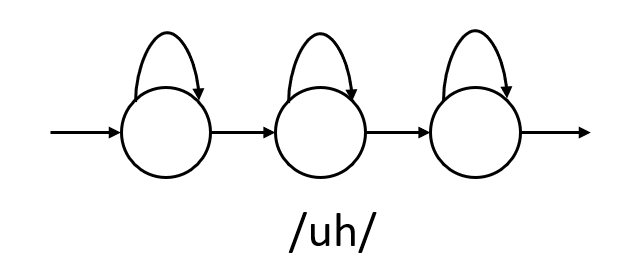
\includegraphics[width=0.45\textwidth]{hmm-uh}
	\caption{音素"/uh/"的HMM\label{fig:hmm-uh}}
\end{figure}

词的HMM可以通过将其连续的音素HMM结合起来形成,比如说单词"cup"的HMM模型如图\ref{fig:hmm-cup}。
\begin{figure}[htbp]
	\centering
	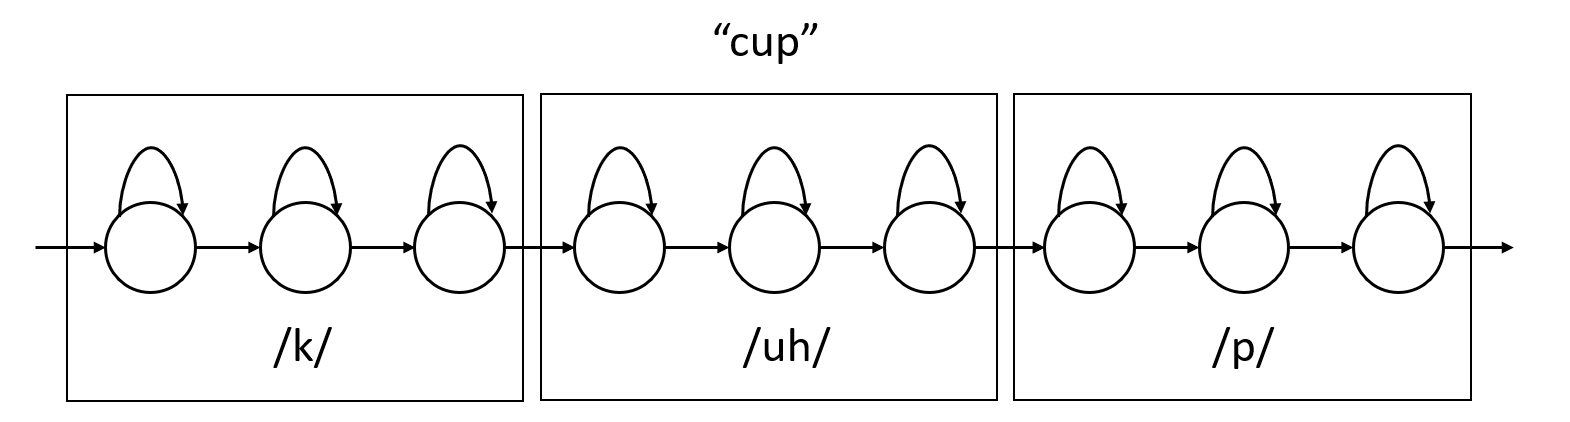
\includegraphics[width=0.50\textwidth]{hmm-cup}
	\caption{单词"cup"的HMM\label{fig:hmm-cup}}
\end{figure}

因此,{\bf 一个高质量的、包含每个单词音素表示的发音词典对于声学模型来说至关重要!}

在HMM-GMM模型中,HMM的状态都有一个概率分布,由GMM建模,其定义如公式\ref{eqn:hmm-gmm}。
\begin{align}
\label{eqn:hmm-gmm}
p(x|s) = \sum_{m} w_m N(x;\mu_{m}, \Sigma_{m})
\end{align}
其中$N(x;\mu_{m}, \Sigma_{m})$是高斯分布,$w_m$是混合权重,其满足$\sum_{m}w_{m}=1$。因此模型每个状态都有自己的GMM。Baum-Welch算法会估计出所有的状态转移概率,以及GMM中的均值、方差和混合权重。

如今语音识别系统中不再使用GMM来对声学观测值建模了,DNN取代了GMM,DNN的输出标签表示的是所有音素的所有状态。比如说有40个音素,每个音素是3-state的HMM,那么DNN的输出就会有$40\times{3}=120$个标签。

这样的声学模型被称作混合模型,即DNN-HMM,其取代了GMM来对声学进行建模。但是HMM其他的部分,尤其是HMM的拓扑结构和转移概率仍然会被用到。

\subsubsection{Choice of Subword Units} % (fold)
\label{ssub:choice_of_subword_units}
我们现在已经知道了如何通过发音词典,链式的绑定音素来形成词HMM。这些音素通常记作"Context Independent" Phones,即CI phones。而事实上单个音素的发音很大程度上依赖于其前面的音素和后面的音素。比如说对于音素"/ah/",在"bat"和"cap"中的发音就是不一样的。

有鉴于此,如果使用"Context-Dependt"(CD) phones,识别的准确率会有很明显的提升。因此对"bat"中,我们用"/b-ah+t/"来表示"/ah/",这样可以得到对应音素的上下文信息;在"cap"中,我们用"/k-ah+p/"来表示"/ah/"。比如说"cup"在句子"a cup of coffee"中,即可用图\ref{fig:hmm-tri}来对单词"cup"建模。
\begin{figure}[htbp]
	\centering
	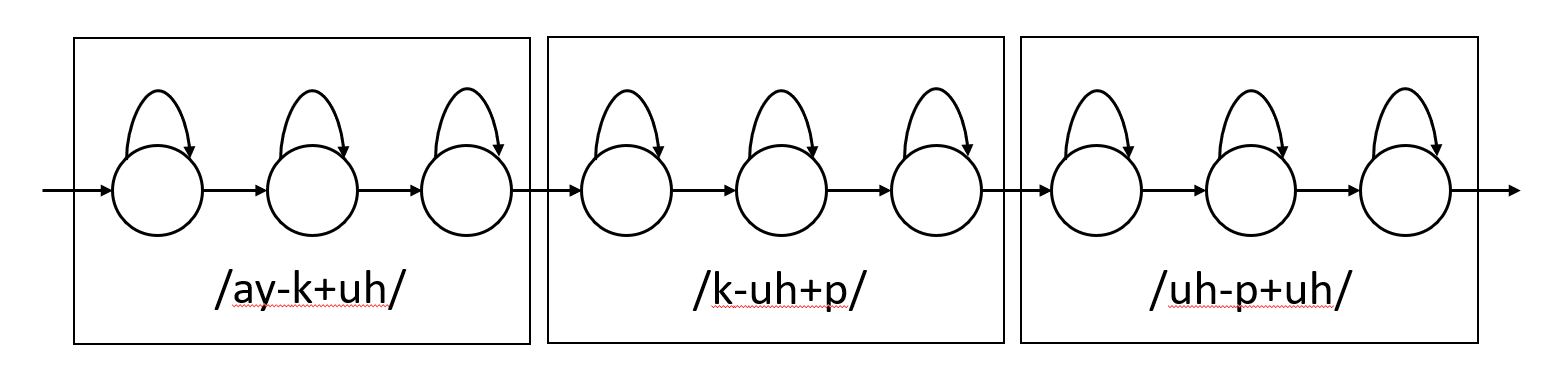
\includegraphics[width=0.50\textwidth]{hmm-tri}
	\caption{单词"cup"的三音素HMM\label{fig:hmm-tri}}
\end{figure}

因为CD phones由三个连续的音素来表示的,记作{\bf triphone}。有的系统用更长的上下文关系来建模,比如"quinphones"就是5个连续的音素表示的,不过这种的不常见。

当ASR使用CI phones来作为声学模型的建模单元时,状态数并不多:$N$个音素乘以每个音素的状态数$P$。美式英语一般有40个音素,每个音素三个状态,那么就有120个CI states。那triphone作为建模单元的话,会有多少个状态呢?triphone有$N^{3}$个,其状态数就有$40^{3}*3=192000$个,这会产生两个很严重的问题:
\begin{enumerate}
	\item 用于训练每一个triphone的数据太少;
	\item 可能有些训练集中没有的triphone,在测试集中出现了。
\end{enumerate}}

广为流传的一种办法是对多个CD states进行池化(pooling),这些CD states具备相似的性质,将它们绑定到一起以形成单个"tied"或者"shared"HMM状态。这些tied states叫做{\bf senone}。这些被绑定的原始状态都通过计算senone的声学分数来得到。

使用决策树(decision tree)将一个集合内的CD triphones states聚类到senones中。对每一个CI phone的每一个状态都会构建一个决策树。

决策树的聚类过程如下:
\begin{enumerate}
	\item 将某个特定状态中,共有中间音素的所有triphone放到一起形成根节点,比如所有满足格式"/*-p+*/"的三音素的第二个状态;
	\item 通过问一系列关于这个三音素的左边context或者右边context的语言学问题使得决策树生长,这些问题都是二选一的问题。比如说:"is the left context phone a back vowel?"或者"is the right context phone voiced?"。在每一个节点,选择训练数据似然度增加最大的问题;
	\item 继续生长,直到节点数达到预设值或者继续分割下去似然度的增加值小于某个阈值;
	\item 决策树的叶子就定义这个CD phone state的senones。
\end{enumerate}

通过决策树聚类生成senones就可以解决上述两大问题,首先,映射成同一个senones的triphone之间可以共享数据,所以其数据的估计也会比较稳定;其次如果测试的时候有个triphone没有出现过,其对应的senone就是顺着决策树搜索,最终找到合适的输出。


几乎所有基于phone的语音识别系统都会使用senone作为包含上下文信息的建模单元。一般工业级的语音识别器大概有10000个senones。这虽然比120个CI state多不少,但是比192000少得多了。

关于决策树的生成,参考RossYoung的博文\upcite{decision},如图\ref{fig:decision-tree}。
\begin{figure}[htbp]
	\centering
	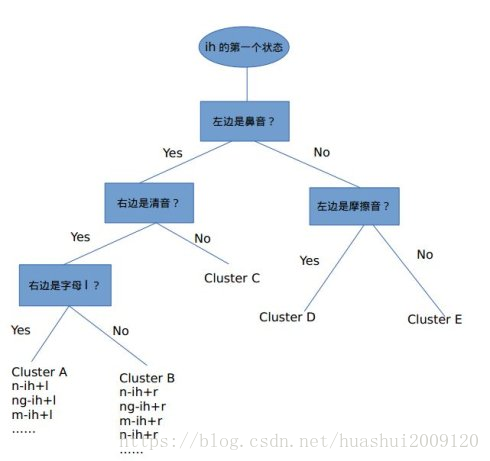
\includegraphics[width=0.45\textwidth]{decision-tree}
	\caption{senones的生成\label{fig:decision-tree}}
\end{figure}

此外,kaldi中的决策树规则是由算法生成的,具体看\ref{sec:kaldi-dt}。

% subsubsection choice_of_subword_units (end)
\subsection{Deep Neural Network Acoustic Models} 
这几年语音识别领域出现的最重要的改进就是使用DNN声学模型。前面也提到过,混合DNN系统使用单个DNN替换了原先的GMMs(每个senone都有一个GMM),DNN的输出标签对应着senones。

训练分类神经网络模型最常用的目标函数是交叉熵(cross entropy),对于一个M类的多分类任务,比如说senones分类,单个样本的目标函数如公式\ref{eqn:dnn-ce}。
\begin{align}
\label{eqn:dnn-ce}
E = -\sum_{m=1}^{M} t_m\log{y_m}
\end{align}

其中$t_m$是标签值(如果这个样本是第$m$类,$t_m$为1,否则为0),$y_m$是网络的实际输出值,神经网络最后一层的输出经过softmax函数映射到概率空间。因此对于每一帧来说,有个$M$维的one-hot向量,其对应的groundtruth,即本帧真真正正对应的senone。

所以,每一帧我们都得给个标签。

为了给所有训练数据的每一帧加上对应senones的标签,我们需要对所有的数据进行强制对齐。强制对齐的操作基本上就是使用HMM模型对每一条语音数据进行解码,限制其解码出来的路径会产生正确的参考文本。强制对齐产生单条最有可能的路径,因此就得到了语句中每一帧对应的senone的标签。

强制对齐操作需要一个语音识别系统,可以是一个基于GMM的初始模型,也可以是一个训练好的DNN模型,但是前提是待对齐的和训练好的模型他们的senones是一样的。

强制对齐的输出文件包含了每一句的起始帧和终止帧,以及对应的senone标签的。不同的工具,这个文件的格式也不一样,以HTK为例,输出是一个MLF格式的文件,如图\ref{fig:htk-force},该文件每一列表示的分别是:
\begin{enumerate}
	\item 开始时间,单位是100ns;
	\item 结束时间,单位是100ns;
	\item Senone的ID;
	\item Senone片段的声学模型得分;
	\item CD triphone HMM 模型;
	\item triphone HMM模型的声学模型得分;
	\item Senone对应文本中的词
\end{enumerate}

\begin{figure}[htbp]
	\centering
	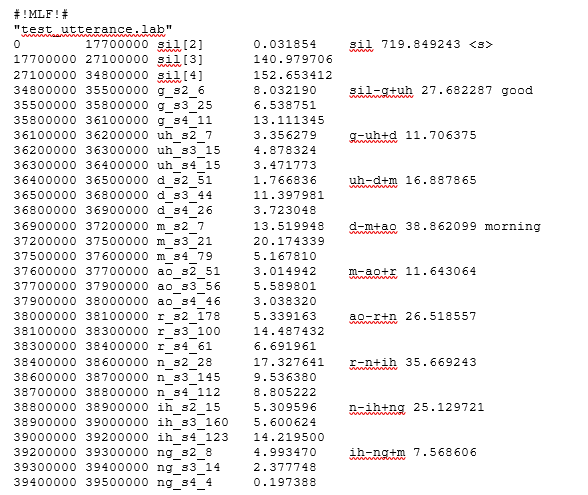
\includegraphics[width=0.7\textwidth]{htk-force}
	\caption{MLF文件示例\label{fig:htk-force}}
\end{figure}

有这样的文件或者类似的文件之后,我们就能得到训练DNN所需的标签了。

\subsection{Training Feedforward Deep Neural Networks} 
构建声学模型的神经网络中,最简单也是最常见的就是前馈神经网络(feed-forward neural network)。前馈神经网络的相关知识网上到处都是,本处咱们只聊基于DNN的声学模型的关键信息。

尽管我们训练一个DNN是为了预测每一个输入帧的标签,如果我们提供一个context window内的帧作为输入的话,而不是使用单独的一帧作为输入,分类的效果会好很多。具体来讲呢,对于$t$时刻的某一帧,DNN的输入是本帧的前N帧、本帧和本帧的后N帧,这个context window是对称的。因此假设$x_t$是$t$时刻的特征向量,那么对应该时刻DNN的输入为:
\begin{align} 
	X_{t} = [x_{t-N}, x_{t-N+1}, ..., x_{t}, ..., x_{t+N-1}, x_{t+N}]
\end{align}

一般呢,$N$的取值范围在5到11之间,这个取决于训练集的体量。越大的context window提供了越多的信息,但是同时会增加输入层的参数矩阵的大小,如果没有足够的数据的话,训练起来会比较困难。

通常还会做一些数据增强,通过加入这些特征的时间导数,记作delta特征。这些特征可以通过简单地差分或者复杂的回归公式计算得到,比如说:
\begin{align}
\begin{split}
\Delta x_{t} &= x_{t+2} - x_{t-2} \\
\Delta^{2} x_{t} &= \Delta x_{t+2} - \Delta x_{t-2} 
\end{split}
\end{align}

这样的话,DNN中每一帧的输入就是一个context window堆叠(stack)的特征,其包含原始的特征向量,delta features和delta-delta features,如下:
\begin{align} 
	x_{t} , \Delta x_{t}, \Delta^{2} x_{t} 
\end{align}

上述的特征经过一系列全连接层,最终通过softmax函数映射成每个senone的概率值,以交叉熵为目标函数,通过BP算法来进行参数的迭代,直到训练结束。整个过程如图\ref{fig:dnn-am}。
\begin{figure}[htbp]
	\centering
	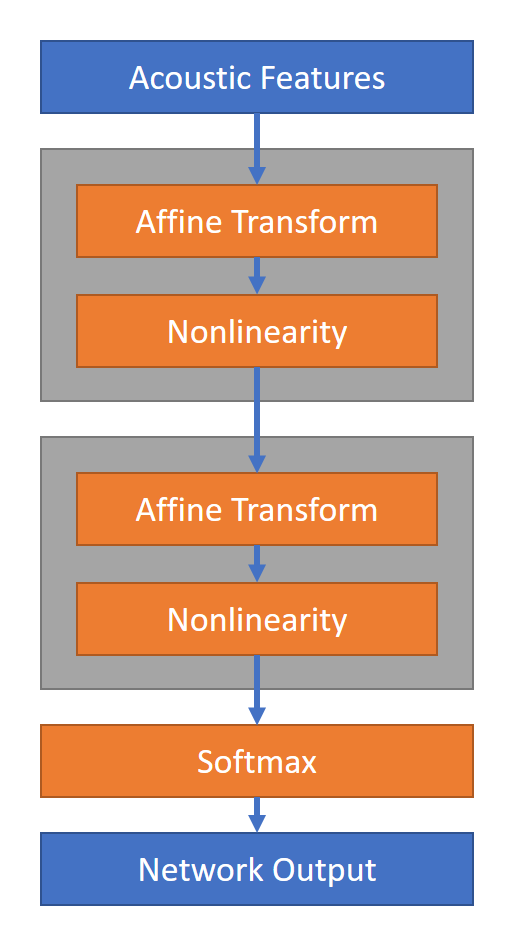
\includegraphics[width=0.2\textwidth]{dnn-am}
	\caption{基于DNN的声学模型训练过程\label{fig:dnn-am}}
\end{figure}

除了基于前馈神经网络的声学模型外,我们经常使用的还有RNN。与DNN不同的是,RNN处理的是序列数据,其权重具备时域依赖性。RNN隐含层的输出如公式\ref{eqn:rnn-am}。
\begin{align} 
\label{eqn:rnn-am}
	h_{t}^{i} = f(W^{i}h_{t}^{i-1} + U^{i}h_{t-1}^{i}+c^{i})
\end{align}
其中$f(\cdot)$是一个非线性函数,比如sigmoid函数或者relu函数,$i$是网络的层数,$t$表示的是帧数或者时间索引,输入$h_{t}^{i-1}$等于第$i-1$层的输出,其实就是上一层的输出,第一层的RNN的输入就等于$x_{t}$。

与DNN相比,循环层的输出既依赖于当前输入,又依赖于上一个时刻的输出。如果你比较熟悉信号处理中的滤波操作,RNN层就可以看作是一个非线性无限脉冲响应(nonlinear infinite impulse response,IIR)滤波器。

对于离线操作的应用来说,延迟并不是很重要的一个指标,所以可以利用双向RNN(bi-RNN)来提升模型的性能。这种情况下,每一层都会有一些参数处理前向序列,同时还会有另一些参数处理后向序列。这样就会有两个输出,将它们拼接(concatenate)到一起作为下一层的输入,如公式\ref{eqn:brnn-am},其中下角标$f$和$b$分别指前向和后向。
\begin{align}
\label{eqn:brnn-am}
\begin{split}
 \overrightarrow{h_{t}^{i}} &= f(W_{f}^{i}h_{t}^{i-1} + U_{f}^{i}h_{t-1}^{i}+c_{f}^{i}) \\
 \overleftarrow{h_{t}^{i}} &= f(W_{b}^{i}h_{t}^{i-1} + U_{b}^{i}h_{t+1}^{i}+c_{b}^{i}) \\
 h_{t}^{i} &= \Big[\overrightarrow{h_{t}^{i}} , \overleftarrow{h_{t}^{i}} \Big]
\end{split}
\end{align}

由于RNN可以学习到特征向量序列之间的时域模式,因此很适合用于声学建模。为了训练RNN,训练序列的序列特性就会保留下来。因此与其用DNN中基于单帧随机化的方式来训练模型,不如采用基于语句随机化的方式。这样的情况下,语句被随机化打乱了,但是语句中的序列特性还是会保留下来。

因为RNN本身的特性决定了模型会学习到数据沿着时间线上的关联关系,就不需要再用一个很宽的context window来捕获每一帧的上下文关系了。对于单向RNN来说,提供一些future context帧是有积极作用的,但是这个数量比DNN要少很多。在双向RNN中,提供context window就失去了意义,因为处理每一帧,网络都可以看到整句的信息,自然会吸收上下文的关联关系。

训练RNN同样使用交叉熵作为目标函数,只是在计算梯度的时候有些微不同。基于这个模型的时域特性,使用BP的变体BPTT算法来更新网络的参数。我们想想看单向RNN的特点,当前时刻的输出不仅依赖于当前输入,还依赖于之前所有时刻的输入。

正如标准的BP算法,BPTT使用梯度下降来优化这个模型,目标函数关于模型参数的梯度是通过链式规则计算得到的,这样导数中就包含了很多梯度的乘积(取决于前面已经处理了多少个时间步)。这些梯度都不存在任何限制,很有可能就会出现梯度接近于0(网络不再学习了)或者接近于无穷大(网络训练就不稳定,也无法收敛)。这个问题就是梯度消失或爆炸。

为了抑制梯度消失的问题,我们一般有两种办法:
\begin{enumerate}
	\item 采用RNN的变体结构,比如LSTM,这个我们一会再说;
	\item 限制BPTT回溯的长度,就是说只允许BPTT利用限定长度的历史信息,这样就会限制连乘梯度的数量。
\end{enumerate}

为了抑制梯度爆炸的问题,可以用gradient clipping(梯度裁剪)的方法。设定一个梯度的上限,对于模型中所有参数的梯度,绝对值超过这个上限的,就让其梯度等于这个上限。

前面提到了LSTM可以抑制梯度消失或爆炸的问题以更好的学习训练集中的长时关系。LSTM中有个概念叫cell,这个东西就是用来存储状态信息的。cell中的信息可以随着时间变化一直被保存着,也可以擦除过去的信息,存入当前的信息。这些操作都依赖于gate来实现。

Gate接近于0,信息就无法通过;Gate接近于1,信息就可以通过。输入门决定了是否将当前时间步的信息存储到cell中;遗忘门决定了是保存cell中信息还是擦掉重写入当前的信息;输出门决定了是否将cell中的信息传出去。LSTM单个神经元的内部如图\ref{fig:lstm-am}。更多关于LSTM的资料参考\upcite{lstm}。
\begin{figure}[htbp]
	\centering
	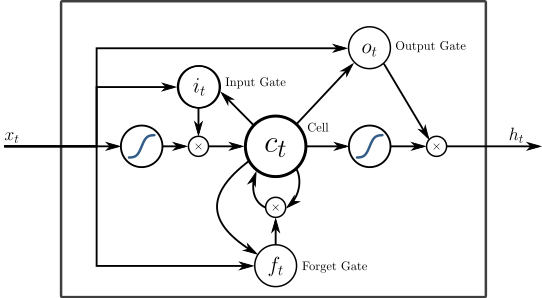
\includegraphics[width=0.5\textwidth]{lstm-am}
	\caption{基于DNN的声学模型训练过程\label{fig:lstm-am}}
\end{figure}

其他的LSTM的变体,比如说GRU,就是LSTM的一个简化版,GRU与LSTM的表现相当,但是参数更少,见\ref{sub:gru}。

\subsection{Using a Sequence based Objective Function} 
RNN是一个序列声学模型,因为它们可以对声学特征向量作为一个时域上连续的序列进行建模。但是其目标函数仍然是帧独立的,就是说在计算目标函数的时候,每一帧的损失是独立计算的。然而因为语音识别是一个序列分类任务,如果我们能搞个基于序列的目标函数,模型的性能应该会有所提升。

GMM-HMM中就有基于序列的目标函数,如今也可以应用于DNN-HMM中。基于帧的交叉熵和序列判别性目标函数的区别就在于基于序列的目标函数更好的对解码过程进行了建模。

具体来说,序列区分性训练中应用了语言模型,来找到那些与参考文本很相似的输出,这些和groundtruth很接近的序列正是网络需要区分开的。相对而言,基于帧的交叉熵作为目标函数,所有不正确的分类都会受到惩罚,即便这些不正确的分类在解码的时候根本不会出现,当然解码的时候需要用的HMM拓扑结构或者语言模型。在序列区分性训练中,正确分类的这些competitors是由解码训练数据得到的。

最常见的一个序列区分性训练目标函数是最大互信息(maximum mutual information, MMI),如公式\ref{eqn:sdt-mmi-edx}。
\begin{align} 
\label{eqn:sdt-mmi-edx}
 F_{MMI} = \sum_{u}\frac{\log{p(X_{u}|S_{u})p(W_{u})}}{\sum_{w^{'}}\log{p(X_{u}|S_{W^{'}})p(W^{'})}}
\end{align}
其中$u$是训练集中句子的索引,$W_u$是语句$u$的参考词序列,$S_u$是对应的状态序列,分母呢是所有可能的词序列的概率和,分母通常由word lattice近似得到,解码的时候word lattice能得到可能输出的词序列。

使用这个目标函数,让声学模型的训练复杂了很多,但是确实能提高识别性能。同样有很多MMI的变体,比如Minimum Phone Error(MPE),和state-level的Minimum Bayes Risk(SMBRa),见\ref{sub:sdt-obj}。

\subsection{Decoding with Neural Network Acoustic Models}
DNN声学模型计算的是在已知声学特征的条件下,某个senone的条件概率,即$p(s|x_t)$,这些state-level的后验概率必须转换成状态的似然度$p(x_t|s)$,只有这样我们才能够使用HMM来解码。如何得到$p(x_t|s)$呢?

根据贝叶斯规则:
\begin{align} 
\label{eqn:bayes-hmm}
	p(x_t|s) = \frac{p(s|x_t)p(x_t)}{p(s)} \propto \frac{p(s|x_t)}{p(s)} 
\end{align}

公式\ref{eqn:bayes-hmm}之所以成立是因为对于所有的senones观测鲜艳$p(x_t)$是个常数,其只是说给似然度增加了个系数而已,因此舍掉它。因此似然度$p(x_t|s)$等于DNN的输出除以senone的先验$p(s)$。而senone的先验可以通过简单地统计训练集中对应senone出现的次数来估计。

上述似然度叫做{\bf scaled likelihood},指代的是其是通过senone的先验scale其后验概率得到的。

\subsection{Lab 3}
{\bf Required files:}
\begin{itemize}
	\item \textcolor{blue}{M3\_Train\_AM.py}
	\item \textcolor{blue}{M3\_Plot\_Training.py}
\end{itemize}}

{\bf Instructions:}

In this lab, we will use the features generated in the previous lab along with the phoneme state alignments provided in the course materials to train two different neural network acoustic models, a DNN and an RNN.

The inputs to the training program are:
\begin{itemize}
	\item {\bf lists/feat\_train.rscp, lists/feat\_dev.rscp} - List of training and dev feature files, stored in a format called RSCP. This standard for relative SCP file, where SCP is HTK-shorthand for script file. It is simply a list of files in the two sets. The dev set is used in training to monitor overfitting and perform early stopping. These files should have been generated as part of completing lab 2.
	\item {\bf am/feat\_mean.ascii, am/feat\_invstddev.ascii} - The global mean and precision (inverse standard deviation) of the training features, also computed in lab 2
	\item {\bf am/labels\_all.cimlf}- The phoneme-state alignments that have been generated as a result of forced alignment of the data to an initial acoustic model. Generating this file requires the construction of a GMM-HMM acoustic model which is outside the scope of this course, so we are providing it to you. The labels for both the training and dev data are in this file.
	\item {\bf am/labels.ciphones}- The list of phoneme state symbols which correspond to the output labels of the neural network acoustic model
	\item {\bf am/ abels\_ciprior.ascii} - The prior probabilities of the phoneme state symbols, obtained by counting the occurences of these labels in the training data.
\end{itemize}

The training, dev, and test RSCP files and the training set global mean and precision files were generated by the lab in Module 2. The remaining files have been provided for you and are in the {\bf am} directory.

{\bf PART1: TRAINING A FEEDFORWARD DNN}

We have provided a python program called {\bf M3\_Train\_AM.py} which will train a feed-forward deep network acoustic model using the files described above. The program is currently configured to train a network with the following hyperparameters:
\begin{itemize}
	\item 4 hidden layers of size 512 hidden units per layer.
	\item 120 output units corresponding to the phoneme states
	\item input context window of 23 frames, which means the input to the network for a given frame is the current frame plus 11 frames in the past and 11 frames in the future
	\item minibatch size of 256
	\item Learning is performed with Momentum SGD with a learning rate of $1e-04$ per sample with momentum as a time constant of 2500
	\item One epoch is defined as a complete pass of the training data and training will run for 100 epochs
	\item The development set will be evaluated every 5 epochs.
\end{itemize}

This can be executed by running:
\begin{lstlisting}[language = python, numbers=left, 
				 numberstyle=\tiny,keywordstyle=\color{blue!70},
				 commentstyle=\color{red!50!green!50!blue!50},frame=shadowbox,
				 rulesepcolor=\color{red!20!green!20!blue!20},basicstyle=\ttfamily]
python M3_Train_AM.py
\end{lstlisting}

On a GTX 965M GPU running on a laptop, the network trained as a rate of 63,000 samples/sec or about 20 seconds per epoch. Thus 100 epochs will run in 2000 seconds or about 30 minutes.

After 100 epochs, the result of training, obtained from the end of the log file, was
\begin{lstlisting}[language = python, numbers=left, 
				 numberstyle=\tiny,keywordstyle=\color{blue!70},
				 commentstyle=\color{red!50!green!50!blue!50},frame=shadowbox,
				 rulesepcolor=\color{red!20!green!20!blue!20},basicstyle=\ttfamily]
Finished Epoch[100 of 100]: [CE_Training] loss = 1.036854 * 1257104, metric = 32.74% * 1257104 17.146s (73317.6 samples/s);
Finished Evaluation [20]: Minibatch[1-11573]: metric = 44.26% * 370331;
\end{lstlisting}

Thus, the training set has a cross entropy of 1.04 per sample, and a 32.74\% frame error rate, while the held-out dev set has a frame error rate of 44.3%

After training is complete, you can visualize the training progress using {\bf M3\_Plot\_Training.py}. It takes a CNTK log file as input and will plot epoch vs. cross-entropy of the training set on one figure and epoch vs. frame error rate of the training and development sets on another figure.
\begin{lstlisting}[language = python, numbers=left, 
				 numberstyle=\tiny,keywordstyle=\color{blue!70},
				 commentstyle=\color{red!50!green!50!blue!50},frame=shadowbox,
				 rulesepcolor=\color{red!20!green!20!blue!20},basicstyle=\ttfamily]
python M3_Plot_Training.py -–log <logfile>
\end{lstlisting}

For this experiment, {\bf <logfile>} would be {\bf ../am/dnn/log}

Here is an example of the figure produced by this script.
\begin{figure}[htbp]
	\centering
	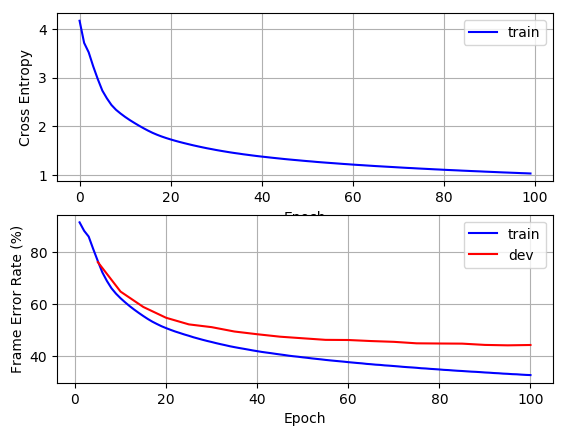
\includegraphics[width=0.6\textwidth]{dnn-ce}
	\caption{DNN声学模型训练图\label{fig:dnn-ce}}
\end{figure}

As you can see from the figure, overfitting has not yet occurred as the development set performance is still the best in the final epoch. It is possible that small additional improvements can be obtained with additional training iterations.

You can now experiment with this neural network training script. You can modify the various hyperparameters to see if the performance can be further improved. For example, you can vary the
\begin{itemize}
	\item Number of layers
	\item Number of hidden units in each layer
	\item Learning rate
	\item Minibatch size
	\item Number of epochs
	\item Learning algorithm (see the CNTK documentation for details on using other learners, such as Adam or AdaGrad)
\end{itemize}

{\bf PART 2: TRAINING A RECURRENT NEURAL NETWORK}

In the second part of this lab, you will modify the code to train a Bidirectional LSTM (BLSTM) network, a type of recurrent neural network.

To train an BLSTM, there are several changes in the code that you should be aware of.
\begin{enumerate}
	\item In DNN training, all frames (samples) are processed independently, so the frames in the training data are randomized across all utterances. In RNN training, the network is trying to learn temporal patterns in the speech sequence, so the order of the utterances can be randomized but the utterances themselves must be kept intact. Thus, we set {\bf frame\_mode=False} in the {\bf MinibatchSource} instantiated by {\bf create\_mb\_source()}.
	\item Change the network creation to create a BLSTM
		\begin{itemize}
			\item In {\bf create\_network()} , we've created a function called {\bf MyBLSTMLayer} as specified below. This function uses the Optimized\_RNN Stack functionality in CNTK. A complete description and additional examples can be found in the CNTK documentation. One thing to be aware of is that with a BLSTM, the size of the hidden layer is actually applied to both directions. Thus, setting the number of hidden units to 512 means that both the forward and backward layers consist of 512 cells. The outputs of the forward and backward layer are then concatenated forming an output of 1024 units. This is then projected back to 512 using the weight matrix W.
\begin{lstlisting}[language = python, numbers=left, 
	 numberstyle=\tiny,keywordstyle=\color{blue!70},
	 commentstyle=\color{red!50!green!50!blue!50},frame=shadowbox,
	 rulesepcolor=\color{red!20!green!20!blue!20},basicstyle=\ttfamily]
def MyBLSTMLayer(hidden_size=128, num_layers=2): 
	W = C.Parameter((C.InferredDimension, hidden_size), init=C.he_normal(1.0), name='rnn_parameters') 
	def _func(operand): 
		return C.optimized_rnnstack(operand, weights=W, hidden_size=hidden_size, num_layers=num_layers, bidirectional=True, recurrent_op='lstm') 
	return _func
\end{lstlisting}
			\item The code calls {\bf MyBLSTMLayer} when the {\bf model\_type} is {\bf BLSTM}. We've reduced the number of hidden layers to 2, since the BLSTM layers have more total parameters than the DNN layers.
		\end{itemize}
	\item For utterance based processing, entire utterance needs to be processed during training. Thus the minibatch size specifies the total number of frames to process but will pack multiple utterances together if possible. Setting the minibatch size to a larger number will allow for efficient processing with multiple utterances in each minibatch size. We have set the minibatch size to 4096.
\end{enumerate}

The traing the BLSTM model, you can execute the following command.
\begin{lstlisting}[language = python, numbers=left, 
	 numberstyle=\tiny,keywordstyle=\color{blue!70},
	 commentstyle=\color{red!50!green!50!blue!50},frame=shadowbox,
	 rulesepcolor=\color{red!20!green!20!blue!20},basicstyle=\ttfamily]
python M3_Train_AM.py –-type BLSTM
\end{lstlisting}

Because of the sequential nature of the BLSTM processing, they are inherently less parallelizable, and thus, train much slower than DNNs. On a GTX 965M GPU running on a laptop, the network trained as a rate of 440 seconds per epoch, or 20 times slower than the DNN. Thus, we will only train for 10 epochs to keep processing time reasonable.

Here too, you can use {\bf M3\_Plot\_Training.py} to inspect the learning schedule in training. And again, if you are interested, you can vary the hyperparameters to try to find a better solution.

%------------------------------------------------------------------------------
%                                Language Modeling
%------------------------------------------------------------------------------
\section{Language Modeling}
\subsection{Introduction} 
本模块介绍语言模型的基础知识。语言模型是语音识别的一个组成部分,其估计的是可能的话语的先验概率$P(W)$。回忆一下前面说过的语音识别的基本公式,这个概率是和声学模型的似然度结合起来以获得最好的输出假设的,如公式\ref{eqn:fund-asr}。
\begin{align}
\label{eqn:fund-asr}
	\hat{W} = \arg\mathop{\max}_{W} P(O|W)P(W)
\end{align}

因此LM表征的是识别器所具备的知识,这个知识表达了可能的词序列是什么,即使这个识别器还没有听到任何实际的音频,因为LM表达的是词序列的先验知识。LM应当给可能的句子高的概率值,不太可能的句子低的概率值,而不是硬性的规定语法语义规则来允许一些句子的存在,不允许另一些句子的存在。LM不应当定下一个绝对的规则是因为没有人知道说话人会说些什么。LM赋予某个句子的概率值也不是通过语言学或者什么规则得到的,它和声学模型一样,来源于数据。因此我们让实际数据的统计学特性来决定在一种语言中,在一个场景中或者在一个应用中,什么词是比较可能出现的。

注意下关于术语的使用,在语言模型中,我们一般把整条音频对应的句子(sentence)称作词序列(word sequence),这里面没有任何暗示表明这个词序列就是一个服从传统语法的、正确的、完整的句子。事实上一个句子的LM针对的是某个场景下说话人可能说出的任何句子。
\subsection{N gram Models}
\subsubsection{Vocabulary}
我们需要给每一个可能的词序列赋予一个概率值:
\begin{align}
	W=w_{1}w_{2}...w_{n}
\end{align}
其中$n$是词的个数,原则上来说这个数量是没有上限的。

首先,我们将问题简化下,用一个有限集合来限制词的可选择空间,即LM的vocabulary。注意LM的vocabulary也就是识别器的vocabulary,我们是没有办法识别一个不被LM包括在内的词的,其概率值无限接近于0的。

vocabulary之外的词呢一般称为是out-of-vocabulary的词,简称OOV。在输入数据中如果存在一个OOV,那么识别器就至少会产生一个错误,所以选择的词典应当最小化OOV出现的可能性。常用的策略是选择出现在训练集中的最频繁的那些词,比如说我们选择训练集中前$N$个出现的最频繁的词或者所有出现次数大于$K$的词,这个$N$或者$K$要选择适当。一般呢最优的词典其大小能够在识别速度和准确率之间找到一个平衡,因为词典越大意味着解码的时候效率越低,而减小OOVs又能提高准确率。当然添加那种基本上不咋出现的词对准确率的影响可以忽略不计,甚至可能降低准确率,因为解码搜索的时候会产生一些错误也会造成声学的模糊性。

\subsubsection{Markov factorization and N-grams}
即便有了一个有限数量的词典,我们同样有无限个词序列,很显然,列举出所有可能的句子是不现实的。就算说我们概念上可以这么干,这样做也没办法去评估LM的参数,因为大部分的句子出现的可能性很小,可能性越小的概率值就得需要更多的数据来评估,这样得到的概率值才是可靠的。

为了解决这两个问题,我们使用一种技巧:使用链式规则将句子的概率值分解成一堆词的概率连乘,如公式\ref{eqn:lm-markov},然后应用马尔科夫假设限制状态和参数的数量。
\begin{align}
\label{eqn:lm-markov}
P(W) = P(w_1)\times{P(w_2|w_1)}\times{P(w_3|w_{1}w_{2})}\times...\times{P(w_n|w_{1}...w_{n-1})} 
\end{align}

如果我们假设是LM是一阶马尔科夫模型,那么我们就可以改写$P(W)$如公式\ref{eqn:lm-markov-1},这就是bigram模型,因为模型只利用了相邻的两个词的统计特性,这样每个词靠前面出现的那个词就可以预测出来。类似的,二阶马尔科夫的LM就称为trigram模型,当前词是靠前面出现的两个词预测出来的。
\begin{align}
\label{eqn:lm-markov-1}
P(W) = P(w_1)\times{P(w_2|w_1)}\times{P(w_3|w_{2})}\times...\times{P(w_n|w_{n-1})} 
\end{align}

这种技巧泛化之后我们就称之为N-gram模型,即当前词依赖于前面出现的$N-1$个词。事实表明trigram比bigram效果要好不少,但是随着$N$的增加,性能提升的就越少。因此实际中我们很少使用超过4-gram或者5-gram以上的LM。实验室一般用的trigram居多,后续讲解我们都以bigram来说明,但是要切记,这些bigram的特点或者bigram的应用都是可以泛化到N-gram的。

\subsubsection{Sentence start and end}
为了让N-gram给所有可能的有限词序列赋予概率,现在有个小问题:模型怎么知道什么时候这个句子结束了呢?我们当然可以搞一个模型来表示句子的长度$n$,但是这样并不方便。我们引入一个特殊的句尾标记</s>用来标记这个句子的结束位置。也就是说LM根据条件分布从左向右生成词,碰到了</s>就停止了。而且,</s>的出现使得所有句子的概率和等于1,详情见\ref{sub:start-end}。

类似地,我们引入句首标记<s>,其位于第一个词$w_1$之前,表示了第一个词的context,这一点至关重要,因为我们希望LM能够学习到第一个词是在句首出现的,比如有些词"I"或者"well"是经常出现在句首的,使用句首标记符号,我们就可以用$P(w_1|<s>)$表示第一个词的bigram概率值。

bigram模型的完整公式如\ref{eqn:bigram-se}。
\begin{align}
\label{eqn:bigram-se}
P(W) = P(w_1|<s>)\times{P(w_2|w_1)}\times{P(w_3|w_{2})}\times...\times{P(w_n|w_{n-1})}\times{P(</s>|w_n)}
\end{align}

\subsubsection{N-gram probability estimation}
N-gram的条件概率可以通过简单地统计频率得到。令$c(w_1,...,w_k)$为k-gram $w_1,..,w_k$出现的次数,比如说词"bites"出现在词"dog"之后的比例为:
\begin{align}\nonumber
P(bites|dog) = \frac{c(dog\ bites)}{c(dog)}
\end{align}

那包含相同context的bigrams概率之和是等于1的。假设context为$<con>$,其在语料库中出现的次数为$c(<con>)=n_0$,而以$<con>$为context的bigrams共有$m$个,分别记作$<con_1>,...,<con_m>$,其出现的次数分别为$n_1,...,n_m$,由此可知:
\begin{align}\nonumber
n_0 = \sum_{i=1}^{m}n_i
\end{align}

每一个bigram的概率值为:
\begin{align}\nonumber
p(<con_i>|<con>)= \frac{n_i}{n_0}
\end{align}

所以所有bigram的概率和为:
\begin{align}\nonumber
\begin{split}
\sum_{i=1}^{m}p(<con_i>|<con>) &= \sum_{i=1}^{m}\frac{n_i}{n_0}  \\
																&= \frac{\sum_{i=1}^{m}n_i}{\sum_{i=1}^{m}n_i}  \\
																&= 1
\end{split}
\end{align}

一般地,k-gram的概率估计如公式\ref{eqn:k-gram}。
\begin{align}
\label{eqn:k-gram}
P(w_k|w_1,...,w_{k-1}) = \frac{c(w_1,...,w_k)}{c(w_1,...,w_{k-1})}
\end{align}

\subsubsection{N-gram smoothing and discounting}
使用相对频率的方式来估计概率值有个很严重的问题:任何在训练集中没有出现的N-gram,其概率值都是0。要知道训练集是有限的,我们不应该仅仅因为有限的语言样本不包含单词组合而排除这些组合,此外,语言并不是一个静态系统,说话人会持续的说出新的表达甚至新的词,要么因为他们有创意,要么语言在交流过程中出错了。

所以我们需要一种原则性的方法将非零概率估计值分配给从来没出现过的N-grams。这个方法就是LM smoothing,我们可以把从未出现过的N-grams看成是模型中的“洞”,我们现在要把洞填平。关于LM的smoothing已经是LM研究的一个分支了,其中的好多方法可以查阅ML wiki中的Smoothing for Language Models\upcite{lmsmoothing},部分LM smoothing算法在SRILM中都有。此处我们详细讨论一种方法:Witten-Bell smoothing。因为其一这个方法好解释也好实现,其二这个方法鲁棒性很好。

Witten-Bell smoothing的思想是把从前未见到的词当成个event,跟那些出现过的词一块计算。训练集中未出现过的词出现了多少次?对于每个独特的词,第一次碰到的时候,这个词就被视作一个新词。对于unigram(上下文无关的),平滑后的概率估计值为:
\begin{align}
\label{eqn:uni-smooth}
\hat{P}(w) = \frac{c(w)}{c(\cdot)+V}
\end{align}
其中$c(w)$是unigram的次数,$c(\cdot)$是词数量的总和(即训练集文本的长度),$V$是第一次碰见"event"的次数,即词典的大小。分母多出来的$V$降低了所有unigram的概率值,因为之前的unigram是通过出现频率计算出来的,因为unigram概率值都下降了,所以LM smoothing也叫做discounting,即N-gram的概率值低于其出现频率。这样就会匀出来部分概率值分给那些未见过的词。Witten-Bell smoothing中未出现的词的概率值为:
\begin{align}
\label{eqn:uni-smooth}
P(unseenword) = \frac{V}{c(\cdot)+V}
\end{align}

我们可以将unigram的情况推广到长度为k的N-gram,前$k-1$个词是第$k$个词的context,然后找到在这个context的条件下出现的独特词类型的数量,如公式\ref{:k-gram-smooth}。
\begin{align}
\label{eqn:k-gram-smooth}
\hat{P}(w_k|w_1...w_{k-1}) = \frac{c(w_{1}...w_{k})}{c(w_{1}...w_{k-1})+V(w_{1}...w_{k-1}\cdot)}
\end{align}
其中$V(w_{1}...w_{k-1}\cdot)$指的是在该context下观测到的词典的大小。同样释放出来的概率值会赋给之前在这个context下没有见过的词。如公式\ref{eqn:k-gram-unseen}。
\begin{align}
\label{eqn:k-gram-unseen}
P(unseenword|w_1...w_{k-1}) = \frac{V(w_{1}...w_{k-1}\cdot)}{c(w_{1}...w_{k-1})+V(w_{1}...w_{k-1}\cdot)}
\end{align}

\subsubsection{Back-off in N-gram models}
在给定一个context条件下,释放出来的那些概率,也就是discounted probability应该如何分配呢?

一种可能的办法是整个词表上均匀分布。比如说context是"white dog",在训练集中,基于这个context的trigram还有一个,"white dog barked",这个trigram出现了两次,那么根据Witten-Bell smoothing,我们可以得到:
\begin{align}\nonumber
\begin{split}
\hat{P}(barked|white\ dog) &= \frac{c(white\ dog\ barked)}{c(white\ dog) + V(white\ dog\cdot)} \\
													 &= \frac{2}{2+1} \\
													 &= \frac{2}{3}
\end{split}
\end{align}

所以释放出来$1/3$的概率给所有其他以"white dog"为context的trigram。这$1/3$的概率值如果均匀分布给这些unseen words就忽略了有些词的出现的频率比其他的高的事实。那么我们可以按照这些词的unigram来给它们分配trigram的概率,但是问题是"white dog the"分配到的概率值比"white dog barks"大得多,因为"the"在语料中出现的次数要比"barks"多得多。更好的办法是使用reduced Context,在这个例子中,我们就用"dog"作为reduced context来算unseen words在原始context下的概率分配。这意味着我们可以统计所有"dog"出现的情况来猜测接下来的词是什么。这个方法叫做回退(back-off),因为碰到没有在full context(2-words)下出现过的词,我们会退回到了更短的context(1-word)下,如公式\ref{eqn:n-gram-backoff}。
\begin{equation}
\label{eqn:n-gram-backoff}
{\hat{P}}_{\text{bo}}\left( w_{k} \right|w_{1}\ldots w_{k - 1}) = \ \left\{ 
\begin{matrix} 
\hat{P}\left( w_{k} \right|w_{1}\ldots w_{k - 1}),\ \ \ c(w_{1}\ldots w_{k}) > 0 \\ 
{\hat{P}}_{\text{bo}}\left( w_{k} \right|w_{2}\ldots w_{k - 1})\ \alpha(w_{2}\ldots w_{k - 1}),\ \  c\left( w_{1}\ldots w_{k} \right) = 0 \\ 
\end{matrix} \right.\
\end{equation}

$\hat{P}_{bo}$是对于所有N-grams的回退估计(back-off estimate),如果N-gram在训练语料中存在,也就是$c(w_{1}\ldots w_{k}) > 0$的时候,就直接使用前面提到的Witten-Bell smoothing计算的概率值$\hat{P}$。如果在训练语料中没有出现过的N-gram,那么就以递归的方式去估计更短的context下的回退概率值,再用系数$\alpha$来量化,$\alpha$是context的函数,也就是词$w_k$在reduced context $w_{2}\ldots w_{k - 1$下的概率值,是依据back-off分布$\hat{P}_{bo}(\cdot|w_{2}\ldots w_{k - 1})$除以$w_k$的概率和,所以所有的$w_k$的估计概率总和为1.

$\alpha$被称为back-off权重,其不是模型的可变参数,一旦N-gram概率$\hat{P}$确定了,$\alpha$就确定下来了。因为要这个权重的作用就是让N-gram的回退概率和为1, $\alpha$的计算也叫做"re-normalizing the model"。

\subsection{Language Model Evalution}
给定两个语言模型A和B,怎么知道哪个模型更好呢?

直觉上来讲,如果模型A赋予测试集(验证集)中存在的词的概率总是比模型B高,那么A就更好一些。因为模型A“浪费”在不会出现的那些词上的概率更少。

对于一个测试集$w_1,...,w_n$,bigram模型输出的概率为:
\begin{align}
P\left( w_{1}\ldots w_{n} \right) = P\left( w_{1}| < s > \right) \times P\left( w_{2} \right|\ w_{1}) \times P\left( w_{3} \right|\ w_{2}) \times \ldots \times P( < /s > \ |\ w_{n})
\end{align}

一个测试集包含多个句子,所以再句子的边界处我们会将context重置为$<s>$。由于连乘的关系,概率值会很小,所以我们换用成对数概率:
\begin{align}
\label{eqn:lm-likelihood}
\log{\ P(w_{1}\ldots w_{n})} = \log{P(w_{1}| < s > )} + \log{P\left( w_{2} \right|\ w_{1})} + \ldots + \log{P( < /s > \ |\ w_{n})}
\end{align}

模型的好坏决定了测试集对数概率的大小,因此我们也把公式\ref{eqn:lm-likelihood}称为对应测试数据的模型对数似然。对数似然只可能是负值,因为概率是小于1的,我们取其相反数,再取个平均值有:
\begin{align}
\label{eqn:lm-op}
-\frac{1}{n} \log P(w_1...w_n)
\end{align}

我们把这个指标称为熵,其是词流的信息率的一种度量。使用LM计算出来的概率,熵可以计算出对词流进行编码所需的平均比特数,越有可能的词所需的比特数越少,所以需要最小化所需的比特率。

另一种评估模型质量的指标是单词概率的平均倒数(the average reciprocal of the word probability),即perplexity(PPL)。如果词的平均概率为$1/100$,那么PPL就是100。作为所讨论的实际模型,PPL是同等可能性单词的词汇量的大小,这些同等可能性单词对于接下来的内容产生相同的不确定性。

怎么去计算PPL呢?

因为模型对于某个数据集的概率是连乘的,所以PPL为词概率连乘的几何平均(geometric aevrage),如公式\ref{eqn:ppl}。
\begin{align}
\label{eqn:ppl}
\sqrt[n]{\frac{1}{P(w_{1}\ldots w_{n})}} = {P(w_{1}\ldots w_{n})}^{- \frac{1}{n}}
\end{align}

PPL就是个熵的对数反函数(指数)。所以这俩指标是等价的。它们的关系为:

HIGH likelihood \leftrightarrow \text{LOW entroy} \leftrightarrow \text{LOW perplexity} \leftrightarrow \text{GOOD model}

LOW likelihood \leftrightarrow \text{HIGH entroy} \leftrightarrow \text{HIGH perplexity} \leftrightarrow \text{BAD model}

需要注意的是使用测试集来评估模型质量应当与训练集是相互独立的,这样才能得到无偏估计。
\subsection{Operations on Language Models}
\subsubsection{N gram Pruning}
N-gram LM有效地记录了训练集中N-grams,因为每个这样的N-gram产生的概率估计都是LM的参数。这么做有个问题,随着训练数据训练的增加,模型的大小随之线性增加。所以有必要去掉那些冗余的参数,比如说back-off机制能在删除高阶N-gram的参数之后还能给出基本一致的结果。实际应用中,我们会通过移除不那么重要的参数来将模型缩小到一定的大小,这样就可以节省存储空间。

我们可以原则性的使用熵或者PPL的概念来进行LM的剪枝。对于模型中的每一个N-gram的概率,我们计算熵或者PPL的变化,如果变化低于某些阈值,就删除掉,或者剪掉这个参数。剪枝之后,模型需要重新归一化,即重新计算back-off权重。

为了让剪枝更贴合实际应用,我们不需要也不想另搞一套测试集来估计这个熵。我们可以使用模型分布所包含的熵,只使用模型包含的信息就使得剪枝标准\upcite{lm-prune}变得简单高效。

\subsubsection{Interporlating Probabilities}
假定有两个已经训练好的LM,其概率估计分别为$\hat{P}_{1}$和$\hat{P}_{2}$。我们怎么样结合这两个模型才能获得一个比较好的N-gram概率呢?

如果可以的话,我们可以重新收集这两个模型的训练数据,扔到一起,然后用这个混合数据训练一个新的模型。但是这样干不方便,还会产生一些别的问题。如果其中一个模型的训练数据比另外一个模型的训练数据多得多,那咋整?比如说哈,其中大的模型是用新闻语料训练的,小的模型是从一个新应用上收集的小数据集训练出来的,如果用混合数据训练一个新的模型,那么大量的、不匹配的新闻数据集就会完全淹没了N-gram的统计特性,这个模型会和预料的应用产生不匹配。

一个更好的办法是以概率来结合这两个模型,通过插入(interpolating)他们的估计。Interpolating就是说我们计算下这两个模型估计的一个非均匀平均,即每个模型的估计值都有一个参数,如公式\ref{eqn:lm-interpolate}。
\begin{align}
\label{eqn:lm-interpolate}
\hat{P}\left( w_{k} \right|w_{1}\ldots w_{k - 1}) = \lambda\ {\hat{P}}_{1}\left( w_{k} \right|w_{1}\ldots w_{k - 1}) + (1 - \lambda)\ {\hat{P}}_{2}\left( w_{k} \right|w_{1}\ldots w_{k - 1})
\end{align}

参数$\lambda$决定了这两个模型的相对影响力,趋近于1则第一个模型为主要模型,趋近于0第二个模型就有更高的权重。$\lambda$的最优值是使用held-out数据计算出的,这些held-out数据与这两个模型的训练数据是分开的。$\lambda$就是能让held-out数据PPL最低的那个值。

Model Interpolation很容易就可以推广到多个模型的情况:M个模型的组合就有M个权重参数,$\lambda_{1},\ \lambda_{2},\ldots,\ \lambda_{M}$,这些参数满足$\lambda_{1} + \ \lambda_{2}, + \ \ldots + \ \lambda_{M} = 1$。和为1的约束条件是为了让Interpolation操作后得到的模型在所有词序列上是归一化的概率值。
\subsubsection{Merging Models}
虽然说不重新训练个模型,model interpolation也能很高效的降低PPL,但是还是有个实际问题存在:我们得始终在磁盘或者内存里保留这些模型,在估计测试集的interpolated模型的时候,对每一个模型进行估计,最终结合这些模型的概率值。

基于back-off的N-gram LM,我们可以构建一个综合N-gram模型,这个模型可以很好地去近似interpolated模型。其算法如\ref{alg:combined-n-gram}。
\begin{algorithm}
\caption{Merged N-gram算法} 
\label{alg:combined-n-gram}
\begin{algorithmic}[1]
\FORALL {for k=1,...,N:}
	\FORALL {  for all ngrams $w_1\ldots{w_k}$}
		\STATE Insert $w_1\ldots{w_k}$ into the new model
		\STATE  Assign probability $\hat{P}(w_k|w_1\ldots{w_{k-1}}$ according to equation \ref{eqn:lm-interpolate}
	\ENDFOR
	\STATE Compute backoff weights for all ngram contexts of length k−1 in the new model
\ENDFOR
\end{algorithmic}
\end{algorithm}

我们在计算$\hat{P}$的时候,其$\hat{P}_{1}$或者$\hat{P}_{1}$可以通过back-off机制获得。

\subsection{Advanced LM Topics}
本节我们来了解下一些比较新的LM建模的算法。LM建模的方法一直都有在研究,但是根据评估\upcite{shen2017},最先进的LM的PPL仍然比人类要差两到三倍,所以任重而道远呀!
\subsubsection{Class-based LM}
N-gram的一个缺点是所有的词都被看作不同的,所以模型需要在训练集中看到足够多次的词才能学到比较好的N-gram。那比如说"Tuesday"和"Wednesday"是语法和意思上都有很多共同点的,那么看到其中一个词N-gram就让我们觉得另一个词的N-gram也存在(看见"store open Tuesday"就会让我们联想到"store open Wednesday"也是可能的N-gram),所以我们应该利用词的相似性来提高LM的泛化能力。

Class-based LM将一些词组起来形成word class,然后以这些类的标签而不是词来统计N-gram的统计特性。比如说我们定义了一个叫"WEEKDAY"的类,其成员为"Monday","Tuesday",...,"Friday",N-gram "store open  Tuesday"就会被当成"store open WEEKDAY"的一个实例。这么干的话,一个纯字符串的概率就等于两个部分乘积:

(1)包含类标签的字符串的概率(以通常的方式计算,类标签是N-gram词汇表的一部分),也就是计算这个实例的N-gram;

(2)类成员的概率,比如说$P(\text{Tuesday}\cup{\text{WEEKDAY}}})$。类成员的概率可以通过数据估计得到,相对于所有的weekday,"Tuesday"出现了多少次,或者直接设置成一个均匀分布,比如说都等于15。

有两种比较基本的办法来得到好的词类。

其中一种使用先验知识,尤其是特定应用领域。比如说要搭建一个旅游应用的语言模型,目的地("Tahiti", "Oslo")、航线以及周几这些实例都应该被覆盖到,甭管说训练数据是不是有这些实体,哪怕训练集中就没有这些实体。我们可以利用类来定义N-gram 模型,比如说"AIRPORT"、"AIRLINE"和"WEEKDAY",用这个类的N-gram来保证这些实例有被覆盖到。这也意味着我们可以通过领域统计特性来设置类成员的的概率,比如说某些旅游景点的受欢迎程度。同时还表示着将词类成员的概率泛化到词组上,比如说"Los Angeles"之于"AIRPORT"。类N-gram的模型框架可以用来推荐词组\upcite{word-phrase-entity}。

另外一种方式是用纯数据驱动的方式来定义词类,这里面不掺杂任何的人类或者领域知识。我们可以搜索所有可能的单词/类映射的空间,并选择一个最小化训练数据上所得到的基于类的模型的PPL(或最大化似然度)。如果想要在合理的时间内搜索到合适的词类,实现细节就很重呀了,详情可以参考一些论文\upcite{class-basedn-gram}。

\subsubsection{Neural Network LMs}
基于神经网络的机器学习算法已经占领了很多领域,比如说语音识别的声学建模等等。同样人工神经网络在LM中也可以用,只要给足够的数据,效果要比N-gram好的多!

DNN之所以能在LM界吃香的喝辣的,因为它搞定了N-gram模型的两大限制。

第一个限制是跨词的泛化不好,前面提到的构建词类就是为了解决这个问题的,但是词类又引入了一个新的问题:多少个词类合适呢?第一个提出的神经网络LM\upcite{lm-nn-bengio}结构叫做前馈LM,其通过一个word embedding层解决了词的泛化问题,word embedding层的作用是将离散的词标签映射到一个密集向量空间。
\begin{figure}[htbp]
	\centering
	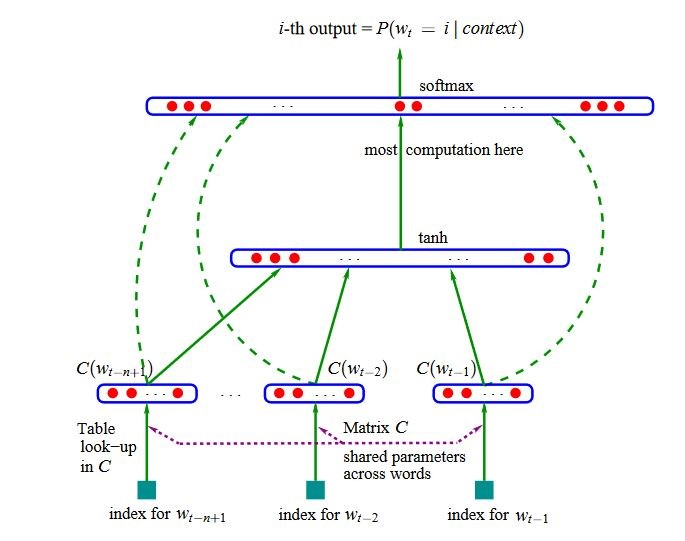
\includegraphics[width=0.5\textwidth]{lm-nn}
	\caption{前馈LM结构图\label{fig:lm-nn}}
\end{figure}

如图\ref{fig:lm-nn}所示,网络的输入是one-hot向量,输入将形成N-gram context的$N-1$个词进行编码,输出是预测随后的词的概率值,输入和输出向量的长度都是词典的大小。所以网络模型就是旧的基于N-gram的LM的直接替代品。关键点是输入的词通过一个共享的矩阵重新编码成了新的向量,这些向量就不再是one-hot形式了,每个输入都会被映射到高维空间。该映射对于所有上下文单词位置是共享的,并且至关重要的是,与下一单词预测器同时进行训练。这种方式的牛逼之处就在于训练好的词嵌入能够用于表征词的相似度,从而来预测词。换句话说,类似地影响下一个单词的上下文单词将被编码为空间中的附近点,然后当遇到新颖组合中的单词时,网络可以利用这种相似性。这是因为所有的网络层都是平滑映射,即相近的输入将会产生类似的输出,事实证明类似于"Tuesday"和"Wednesday"的词他们的嵌入向量有着相似性。

N-gram的另外一个限制时其截断上下文,它总是总是限制在前面的$N-1$个单词。问题在于,语言允许在相关的单词之间嵌入子句、任意长的形容词列表以及任意距离的其他结构,而这些被分隔开的词在预测下一个词的时候是有用的。任何合理的$N$都没办法在一个context中捕捉所有的可预测的单词。这种限制由RNN解决,RNN将某个隐含层在$t-1$时刻的激活值作为额外的输出送给下一个时刻$t$,如图\ref{fig:lm-rnn}。
\begin{figure}[htbp]
	\centering
	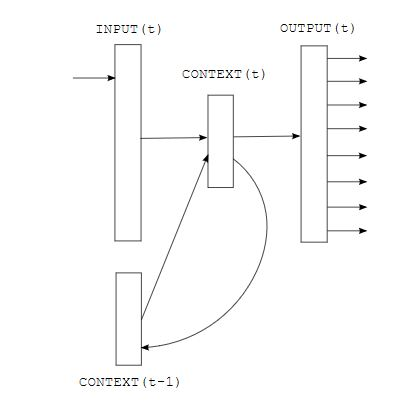
\includegraphics[width=0.4\textwidth]{lm-rnn}
	\caption{RNNLM结构图\label{fig:lm-rnn}}
\end{figure}

RNNLM允许重复性的将某个词位置的信息传递给下一个词,不存在关于词之间间隔距离的硬性限制,所以很远位置的词信息也可以用于预测当前时刻的此预测。当然RNN本身结构存在的一些缺陷,梯度消失或者梯度爆炸都可以用门信息流的RNN变体来解决,常见的用LSTM和GRU等。

前馈LM和RNNLM都随着神经网络的发展而获得更好的效果,比如说更深层的网络和更好的训练方式。基于神经网络的LM还有另外一个趋势是对字而不是词单元进行建模。很明显,人工神经网络在高级信息流方面为模型架构进行试验提供了很大的灵活性,我们不必担心编码和概率分布的详细设计,其已经大大推进了该领域的发展,未来必将有更多的发展。
\subsection{Lab 4: Language Modeling}
{\bf \textcolor{gray}{INTRODUCTION AND SETUP}}

In this lab, we will practice the main techniques for building N-gram based language models for our speech recognizer. In subsequent modules, the resulting LM will be used in the speech recognition decoder, together with the acoustic model from the preceding lab.

This lab is carried out in a Linux command shell environment. The get started, make sure you know how to invoke the Linux bash shell, either on a native Linux system, using Cygwin on a Windows system, or in the Windows subsystem for Linux. Bash is the default shell on most systems.

Inside bash, change into the M4\_Language\_Modeling directory:
\begin{itemize}
	\item cd M4\_Language\_Modeling
\end{itemize}

We will be using pre-built executables from the SRI Language Modeling toolkit (\href{http://www.speech.sri.com/projects/srilm/}{SRILM}). Start by adding the SRILM binary directories to your search path. If you are in a Cygwin,
\begin{itemize}
	\item PATH=\$PWD/srilm/bin/cygwin64:\$PWD/srilm/bin:\$PATH
\end{itemize}

In Linux or Windows Subsystem for Linux, use
\begin{itemize}
	\item PATH=\$PWD/srilm/bin/i686-m64:\$PWD/srilm/bin:\$PATH
\end{itemize}

You can put this command in the .bashrc file in your home directory, so it is run automatically next time you invoke the shell. Also, make sure you have the \href{http://man7.org/linux/man-pages/man1/gawk.1.html}{gawk} utility installed on your system. As a check that all is set up, run
\begin{itemize}
	\item ngram-count -write-vocab –
	\item compute-oov-rate < /dev/null
\end{itemize}

which should each output a few lines of text without error messages. It will be helpful to also install the optional wget command.

Since language modeling involves a fair amount of text processing it will be useful to have some familiarity with Linux text utilities such as \href{http://man7.org/linux/man-pages/man1/sort.1.html}{sort}, head, \href{http://man7.org/linux/man-pages/man1/wc.1.html}{wc}, \href{http://man7.org/linux/man-pages/man1/sed.1.html}{sed}, \href{http://man7.org/linux/man-pages/man1/gawk.1.html}{gawk} or \href{https://perldoc.perl.org/perl.html}{perl}, and others, as well as Linux mechanisms for redirecting command \href{https://en.wikipedia.org/wiki/Standard_streams}{standard input/output}, and \href{https://en.wikipedia.org/wiki/Pipeline_\%28Unix\%29}{pipelining} several commands. We will show you commands that you can copy into the shell to follow along, using this symbol
\begin{itemize}
	\item command argument1 argument2 …
\end{itemize}

but we encourage you try your own solutions to achieve the stated goals of each exercise, and to explore variants.

{\bf \textcolor{gray}{PREPARING THE DATA}}

We will be using the transcripts of the acoustic development and test data as our dev and test sets for language modeling.

{\bf TASK:} Locate files in the 'data' subdirectory and count the number of lines and words in them.

{\bf SOLUTION:}
\begin{itemize}
	\item ls data
	\item wc -wl data/dev.txt data/test.txt
\end{itemize}

{\bf TASK:} View the contents of these files, using your favorite pager, editor, or other tool. What do you notice about the format of these files? How do they differ from text you are used to?

{\bf SOLUTION:}
\begin{itemize}
	\item head data/*.txt
\end{itemize}

You will notice that the data is in all-lowercase, without any punctuation. This is because we will model sequences of words only, devoid of textual layout, similar to how one your read or speak them. The spelling has to match the way words are represented in the acoustic model. The process of mapping text to the standard form adopted for modeling purposes is called text normalization (or TN for short), and typically involves stripping punctuation, mapping case, fixing typos, and standardizing spellings of words (like MR. versus MISTER). This step can consume considerable time and often relies on powerful text processing tools like sed or perl.

Because it is so dependent on the source of the data, domain conventions, and tool knowledge, we will not elaborate on it here. Instead, we will download an LM training corpus that has already been normalized,
\begin{itemize}
	\item wget \url{http://www.openslr.org/resources/11/librispeech-lm-norm.txt.gz}
\end{itemize}

If your system doesn’t have the wget command you can download this file in a browser and move it into the LM lab directory.

{\bf TASK:} Inspect the file and count lines and word tokens. How does the text normalization of this file differ from our test data?

{\bf SOLUTION:} The file is compressed in the gzip (.gz) so we must use the \href{https://www.gnu.org/software/gzip/manual/gzip.html}{gunzip} tool
\begin{itemize}
	\item gunzip -c librispeech-lm-norm.txt.gz | head
	\item gunzip -c librispeech-lm-norm.txt.gz | wc -wl
\end{itemize}

The second command can take a while as the file is large. You will notice that this file is text normalized but uses all-uppercase instead of all-lowercase.

Language model training data, and language models themselves, are often quite large but compress well since they contain text. Therefore, we like to keep them in compressed form. The SRILM tools know how to read/write .gz files, and it is easy to combine gzip/gunzip with Linux text processing tools.

{\bf OPTIONAL TASK:} Download the raw training data at \url{http://www.openslr.org/12/librispeech-lm-corpus.tgz}, and compare it to the normalized text. How would you perform TN for this data?

{\bf SOLUTION:} left to the readers!

{\bf \textcolor{gray}{DEFINING A VOCABULARY}}

The first step in building a LM is to define the set of words that it should model. We want to cover the largest possible share of the word tokens with the smallest set of words, so as to keep model size to a minimum. That suggests picking the words that are most frequent based on the training data.

One of the functions of the \href{http://www.speech.sri.com/projects/srilm/manpages/ngram-count.1.html}{ngram-count} tool is to count word and ngram occurrences in a text file.
\begin{itemize}
	\item ngram-count -text TEXT -order 1 -write COUNTS -tolower
\end{itemize}

Will count 1-grams (i.e., words) and write the counts to a file. The final option above maps all text to lowercase, thus dealing with the mismatch we have between our training and test data.

{\bf TASK:} Extract the list of the 10,000 most frequent word types in the training data. What kinds of words do you expect to be at the top of the list? Check your intuition.

{\bf HINT:} Check out the Linux sort, head, and cut commands.

{\bf SOLUTION:}
\begin{itemize}
	\item ngram-count -text librispeech-lm-norm.txt.gz -order 1 -write librispeech.1grams -tolower
	\item sort -k 2,2 -n -r librispeech.1grams | head -10000 > librispeech.top10k.1grams
	\item cut -f 1 librispeech.top10k.1grams | sort > librispeech.top10k.vocab
\end{itemize}

The intermediate file librispeech.top10k.1grams contains the words and their counts sorted most frequent first. As you might expect, common function words liked “the”, “and”, “of” appear at the top of the list. Near the top we also find two special tags, $<s>$ and $</s>$. These are added by ngram-count to mark the start and end, respectively, of each sentence. Their count equals the number of non-empty lines in the training data, since it is assumed that each line contains one sentence (empty lines are ignored).

We now want to find out how well out 10k vocabulary covers the test data. We could again use Linux tools for that, but SRILM contains a handy script \href{http://www.speech.sri.com/projects/srilm/manpages/training-scripts.1.html}{compute-oov-rate} that takes two arguments: the unigram count file and the list of vocabulary words.

{\bf TASK:} What is the rate of out-of-vocabulary (OOV) words on the training, dev and test sets?

{\bf HINT:}  Use the same method as before to generate the unigrams for dev and test data.

{\bf SOLUTION:}
\begin{itemize}
	\item compute-oov-rate librispeech.top10k.vocab
	\item ngram-count -text data/dev.txt -order 1 -write dev.1grams
	\item compute-oov-rate librispeech.top10k.vocab dev.1grams
	\item ngram-count -text data/test.txt -order 1 -write test.1grams
	\item compute-oov-rate librispeech.top10k.vocab test.1grams
\end{itemize}

Usually we expect the OOV rate to be lowest on the training set because we used it to select the words (the vocabulary is biased toward the training set), but in this case the test sets have been chosen to be “cleaner” and have lower OOV rates. (The training data actually contains some languages other than English, though most of those will not make it into the vocabulary.)

Note that compute-oov-rate also reports about “OOV types”. OOV types are the number of unique words that are missing from the vocabulary, regardless of how many times they occur.

The OOV rate of around 5\% is quite high – remember that we will never be able to recognize those OOV words since the LM does not include them (they effectively have probability zero). However, we chose the relatively small vocabulary size of 10k to speed up experiments with the decoder later.

{\bf OPTIONAL TASK}: Repeat the steps above for different vocabulary sizes (5k, 20k, 50k, 100k, 200k). Plot the OOV rate as a function of vocabulary size. What shape do you see?

{\bf \textcolor{gray}{TRAINING A MODEL}}

We are now ready to build a language model from the training data and the chosen vocabulary. This is also done using the ngram-count command. For instructional purpose we will do this in two steps: compute the N-gram statistics (counts), and then estimate the model parameters. (ngram-count can do both in one step, but that’s not helpful to understand what happens under the hood.)

{\bf TASK:} Generate a file containing counts of all trigrams from the training data. Inspect the resulting file

{\bf HINT:}  Consult the \href{http://www.speech.sri.com/projects/srilm/manpages/ngram-count.1.html}{ngram-count} man page and look up the options -order, -text, and -write. Remember the case mismatch issue.

{\bf SOLUTION: The first command uses about 10GB of memory and takes 15 minutes on a 2.4GHz Intel Xeon E5 CPU, so be sure to procure a sufficiently equipped machine and some patience.}
\begin{itemize}
	\item ngram-count -text librispeech-lm-norm.txt.gz -tolower -order 3 -write librispeech.3grams.gz
	\item gunzip -c librispeech.3grams.gz | less
\end{itemize}

Note that we want to compress the output file since it is large. The -order option in this case is strictly speaking optional since order 3 is the default setting. Note that the output is grouped by common prefixes of N-grams, but that the words themselves are not alphabetically sorted. You can use the -sort option to achieve the latter.

Now we can build the LM itself. (Modify the output file names from previous steps according to your own choices.)

{\bf TASK:} Estimate a backoff trigram LM from librispeech.3grams.gz, using the Witten-Bell smoothing method.

{\bf HINT:}  Consult the ngram-count man page for options -read, -lm, -vocab, and -wbdiscount .

{\bf SOLUTION:}
\begin{itemize}
	\item ngram-count -debug 1 -order 3 -vocab librispeech.top10k.vocab -read librispeech.3grams.gz -wbdiscount -lm librispeech.3bo.gz
\end{itemize}

We added the -debug 1 option to output a bit of information about the estimation and resulting LM, in particular the number of N-grams output.

We will now try to understand the way LM parameters are stored in the model file. Peruse the file using
\begin{itemize}
	\item gunzip -c librispeech.3bo.gz | less
\end{itemize}

or, if you prefer, gunzip the entire file using
\begin{itemize}
	\item gunzip librispeech.3bo.gz
\end{itemize}

and open librispeech.3bo in an editor. Note: the editor better be able to handle very large files – the LM file has a size of 1.3 GB.

{\bf \textcolor{gray}{Model evaluation}}

Consult the description of the backoff LM file format \href{http://www.speech.sri.com/projects/srilm/manpages/ngram-format.5.html}{ngram-format(5)}, and compare to what you see in our model file, to be used in the next task.

{\bf TASK:} Given the sentence “a model was born”, what is the conditional probability of “born”?

{\bf HINT:}  Consult the ngram-count man page for options -read, -lm, -vocab, and -wbdiscount .

{\bf SOLUTION:} The model is a trigram, so the longest N-gram that would yield a probability to predict “born” would be “model was born”. So let’s check the model for that trigram. (One way to locate information in the model file is the zgrep command, which searches a compressed file for text strings. Each search string below starts with a TAB character to avoid spurious matches against other words that contain the string as a suffix. You can use your favorite tools to perform these searches.)
\begin{itemize}
	\item zgrep " model was born" librispeech.3bo.gz
\end{itemize}

This outputs nothing, meaning that trigram is not found in the model, and we have to use the back-off mechanism. We look for the line that contains the context bigram “model was” following a whitespace character:
\begin{itemize}
	\item zgrep -E “\smodel was” librispeech.3bo.gz | head -1

			-2.001953 model was 0.02913048
\end{itemize}

The first number is the log probability $P(was | model)$, which is of no use to use here. The number at the end is the backoff weight associated with the context “model was”. It, too, is encoded as a base-10 logarithm. Next, we need to find the bigram probability we’re backing off to, i.e., $P(born | was)$:
\begin{itemize}
	\item zgrep -E “\swas born” librispeech.3bo.gz | head -1

			-2.597636 was born -0.4911189
\end{itemize}

The first number is the bigram probability $P(born | was)$. We can now compute the log probability for $P(born | model was)$ as the sum of the backoff weight and the bigram probability:

$0.02913048 + -2.597636 = -2.568506$ or as a linear probability $10^{-2.568506} = 0.002700813$.

{\bf TASK:} Compute the total sentence probability of “a model was born” using the ngram -ppl function. Verify that the conditional probability for “born” is as computed above.

{\bf SOLUTION:} We feed the input sentence to the ngram command in a line of standard input, i.e., using “-“ as the filename argument to -ppl. Use the option -debug 2 to get a detailed breakdown of the sentence-level probability:
\begin{itemize}
	\item echo “a model was born” | ngram -debug 2 -lm librispeech.3bo.gz -ppl –
\begin{lstlisting}[language = python, numbers=left, 
	 numberstyle=\tiny,keywordstyle=\color{blue!70},
	 commentstyle=\color{red!50!green!50!blue!50},frame=shadowbox,
	 rulesepcolor=\color{red!20!green!20!blue!20},basicstyle=\ttfamily]
a model was born

p( a | <s> ) =
2gram
0.01653415
−1.781618

p( model | a …) =
3gram
0.0001548981
−3.809954

p( was | model …) =
3gram
0.002774693
−2.556785

p( born | was …) =
2gram
0.002700813
−2.568506

p( </s> | born …) =
3gram
0.1352684
−0.8688038

1 sentences, 4 words, 0 OOVs

0 zeroprobs, logprob= -11.58567 ppl= 207.555 ppl1= 787.8011
\end{lstlisting}

\end{itemize}

Notice how ngram adds the sentence start and end tags, <s> and </s>. The final line gives both the log probability and the perplexity of the entire sentence. The line starting "$p(born | was …)$" has the conditional word probability that we computed previously. The label "2gram" indicates that a backoff to bigram was used. The final “logprob” value $-11.58567$ is just the sum of the log probabilities printed for each word token. Let’s verify the perplexity value based on it’s definition: we divide the logprob by the number of word tokens (including the end-of-sentence), convert to a probability and take the reciprocal (by negating the exponent): $10^{\frac{11.58567}{5}}= 207.555$. Of course this is not a good estimate of perplexity as it is based on only 5 data points.

{\bf TASK:} Compute the perplexity of the model over the entire dev set.

{\bf SOLUTION:} The exact same invocation of ngram can be used, except we use the file containing the dev set as ppl input. We also omit the -debug option to avoid voluminous output. Note: these commands take a few seconds to run, only because loading the large LM file into memory takes some time – the model evaluation itself is virtually instantaneous.
\begin{itemize}
	\item ngram -lm librispeech.3bo.gz -ppl data/dev.txt

			file dev.txt: 466 sentences, 10841 words, 625 OOVs

			0 zeroprobs, logprob= -21939 ppl= 113.1955 ppl1= 140.4475
\end{itemize}

We thus have a perplexity of about 113. The first line of summary statistics also gives the number of out-of-vocabulary words (which don’t count toward the perplexity, since they get probability zero). In this case the OOV rate is 625/10841 = 5.8%.

Running the same command on the test set (data/test.txt) yields a perplexity of 101 and an OOV rate of 4.9\%. Both statistics indicate that the test portion of the data is a slightly better match to our model than the development set.

{\bf TASK:} Vary the size of the training data and observe the effect this has on model size and quality (perplexity).

{\bf HINT:} The original librispeech-lm-norm.txt.gz has about 40 million lines. Use gunzip and the head command to prepare training data that is $\frac{1}{2}$, $\frac{1}{4}$, …, of the full size. (This is very easy, but can you think of better ways to pare down the data?)

{\bf SOLUTION:} Rebuild the model (using the original vocabulary), and evaluate perplexity for different amounts of data. Plot model size (number of ngrams in the head of the model file) and perplexity as a function of training data size. Details left to the student, using the steps discussed earlier.

{\bf \textcolor{gray}{Model adaptation}}

We will now work through the steps involved in adapting an existing LM to a new application domain. In this scenario we typically have a small amount of training data for the new, target domain, but a large amount, albeit mismatched data from other sources. For this exercise we target the \href{http://www.amiproject.org/}{AMI domain} of multi-person meetings as our target domain. The language in this are spontaneous utterances from face-to-face interactions, whereas the “librispeech” data we used so far consisted of read books, a dramatic mismatch in speaking styles and topics.

We will use the “librispeech” corpus as our out-of-domain data, and adapt the model we just created from that corpus to the AMI domain, using a small amount of target-domain data corpus. Corpus subsets for training and test are in the data directory:
\begin{itemize}
	\item wc -wl data/ami-*.txt

			6473 data/ami-dev.txt

			2096 20613 data/ami-test.txt

			86685 924896 data/ami-train.txt
\end{itemize}

Also provided is a target domain vocabulary consisting of all words occurring at least 3 times in the training data, consisting of 6171 words:
\begin{itemize}
	\item wc -l data/ami-train.min3.vocab

			6271 data/ami-train.min3.vocab
\end{itemize}

{\bf TASK:} Build the same kind of Witten-Bell-smoothed trigram model as before, using the provide AMI training data and vocabulary. Evaluate its perplexity on the AMI dev data.

{\bf SOLUTION:}
\begin{itemize}
	\item ngram-count -text data/ami-train.txt -tolower -order 3 -write ami.3grams.gz
	\item ngram-count -debug 1 -order 3 -vocab data/ami-train.min3.vocab -read ami.3grams.gz -wbdiscount -lm ami.3bo.gz
	\item ngram -lm ami.3bo.gz -ppl data/ami-dev.txt

			file data/ami-dev.txt: 2314 sentences, 26473 words, 1264 OOVs

			0 zeroprobs, logprob= -55254.39 ppl= 101.7587 ppl1= 155.5435
\end{itemize}

{\bf TASK:} Evaluate the previously built librispeech model on the AMI dev set.

{\bf SOLUTION:} Again, this takes a few seconds due to the loading time of the large model.
\begin{itemize}
	\item ngram -lm librispeech.3bo.gz -ppl data/ami-dev.txt

			file data/ami-dev.txt: 2314 sentences, 26473 words, 3790 OOVs

			0 zeroprobs, logprob= -56364.05 ppl= 179.8177 ppl1= 305.3926
\end{itemize}

Note how both the perplexity and the OOV count are substantially higher for this large model than for the much small, but well-matched AMI language model. If we modified the vocabulary of the old model to match the new domain its perplexity would increase further. (Can you explain why?)

We will now adapt the old model by interpolating it with the small AMI LM. As explained in the course materials, model interpolation means that all N-gram probabilities are replaced by weighted averages of the two input models. So we need to specify the relative weights of the two existing models, which must sum to 1. A good rule of thumb is to give the majority of weight (0.8 or 0.9) to the in-domain model, leaving a small residual weight (0.2 or 0.1) to the out-of-domain model.

{\bf TASK:} Construct an interpolated model based on the existing librispeech and AMI models, giving weight 0.8 to the AMI model, and evaluate it on the dev set.

{\bf HINT:} Make use of the ngram options -mix-lm, -lambda, and -write-lm.
\begin{itemize}
	\item ngram -debug 1 -order 3 -lm ami.3bo.gz -lambda 0.8 -mix-lm librispeech.3bo.gz -write-lm ami+librispeech.bo.gz
	\item ngram -lm ami+librispeech.3bo.gz -ppl data/ami-dev.txt

			file ami-dev.txt: 2314 sentences, 26473 words, 783 OOVs

			0 zeroprobs, logprob= -56313.77 ppl= 102.546 ppl1= 155.6145
\end{itemize}

At first sight, this result is disappointing. Note how the perplexity is now 102, slightly up from the value that the AMI-only model produced. But also note how the number of OOVs was almost halved (from 1264 to 783), due to the addition of words covered by the out-of-domain model that were not in the AMI model. The model now has more words to choose from when making its predictions. An important lesson from this exercise is that we can only compare perplexity values when the underlying vocabularies are the same. Otherwise, the enlarged vocabulary is a good thing, as it reduces OOVs. The interpolation step has effectively adapted not only the model probabilities, but the vocabulary as well.

Still, it would be nice to do an apples-to-apples comparison to see the effect of just the probability interpolation on model perplexity. We can do this by telling the ngram tool to only use words from the AMI vocabulary in the interpolated model:
\begin{itemize}
	\item ngram -debug 1 -order 3 -lm ami.3bo.gz -lambda 0.8 -mix-lm librispeech.3bo.gz -write-lm ami+librispeech.bo.gz -vocab data/ami-train.min3.vocab -limit-vocab
\end{itemize}

This is the same command as before, but with the -limit-vocab option added, telling ngram to only use the vocabulary specified by the -vocab option argument. We can now evaluate perplexity again:

file ami-dev.txt: 2314 sentences, 26473 words, 1264 OOVs

0 zeroprobs, logprob= -53856.04 ppl= 90.52426 ppl1= 136.8931

The number of OOVs is now back to the same as with ami.3bo.gz, but perplexity is reduced from 102 to 90.

{\bf TASK (optional):} Repeat this process for different interpolation weights, and see if you can reduce perplexity further. Check results on both AMI dev and test sets.

This step is best carried out using the enlarged vocabulary, since that is what we want to use in our final model. But notice how we are now effectively using the dev set to train another model parameter, the interpolation weight. The result will thus be tuned to the dev set. This is why we better have another test set held out (data/ami-test.txt in this case) to verify that the result of this tuning also improves the model (lowers the perplexity) on independent data.

The tuning of interpolation weights would be rather tedious if carried out by trial and error. Fortunately, there is an efficient algorithm that finds optimal weights based on \href{https://en.wikipedia.org/wiki/Expectation\%E2\%80\%93maximization\_algorithm}{expectation maximation}, implemented in the command compute-best-mix, described under \href{http://www.speech.sri.com/projects/srilm/manpages/ppl-scripts.1.html}{ppl-scripts}.

TASK (optional): Use compute-best-mix to find the best -lambda value for interpolation for the two models we built.

{\bf HINT:} As input to the command, generate detailed perplexity output for both models, using ngram -debug 2 -ppl data/ami-dev.txt .

{\bf \textcolor{gray}{Model pruning}}

We saw earlier that model size (and perplexity) varies with the amount of training data. However, if a model gets too big for deployment as the data size increases it would be a shame to have to not use it just for that reason. A better approach is to train a model on all available data, and then eliminate parameters that are redundant or have little effect on model performance. This is what model pruning does.

A widely used algorithm for model pruning based on entropy is implemented in the ngram tool. The option -prune takes a small value, such as $10^{-8}$ or $10^{-9}$, and remove all ngrams from the model that (by themselves) raise the perplexity of the model less than that value in relative terms.

{\bf TASK:} Shrink the large librispeech model trained earlier, using pruning values between $10^{-5}$ and $10^{-10}$ (stepping by powers of ten). Observe/plot the resulting model sizes and perplexities, and compare to the original model.

{\bf SOLUTION:} Starting with $1e-5$ (= $10^{-5}$ in floating point notation), create the pruned model:
\begin{itemize}
	\item ngram -debug 1 -lm librispeech.3bo.gz -prune 1e-5 -write-lm librispeech-pruned.3bo.gz
\end{itemize}

Then evaluate the librispeech-pruned.3bo.gz model on the entire dev set, as before. The -debug option lets the tool output the number of ngrams pruned and written out. Add the resulting number of bigrams and trigrams to characterize the pruned model size (roughly, the number of model parameters, since the number of unigrams is fixed to the vocabulary, and the backoff weights are determined by the probability parameters).











%------------------------------------------------------------------------------
%                                Speech Decoding
%------------------------------------------------------------------------------
\section{Speech Decoding}
\subsection{Overview}

\subsection{Weighted Finite State Transducers}

\subsection{WFSTs and Acceptors}

\subsection{Graph Composition}

\subsection{Lab 5}


%------------------------------------------------------------------------------
%                                Advanced Acoustic Modeling
%------------------------------------------------------------------------------
\section{Advanced Acoustic Modeling}
\subsection{Imporved Objective Functions}

\subsection{Sequential Objective Function}

\subsection{Connectionist Temporal Classsification}

\subsection{Sequence Discriminative Objective Functions}

\subsection{Lab 6}


\section{补充知识点}

\subsection{傅里叶变换}

\subsection{Nyquist定理}

\subsection{编辑距离}
\label{sub:edit-distance}
本节分析参考的是明无梦的blog\upcite{mingwumeng}。
{\bf Description:}

给定2个字符串a,b,编辑距离是将a转换为b的最少操作次数,其操作只允许以下三种:
\begin{enumerate}
	\item 插入一个字符(Insert):例如 $fj\rightarrow{fxj}$;
	\item 删除一个字符(Delete):例如 $fxj\rightarrow{fj}$;
	\item 替换一个字符(Substitue):例如 $jxj\rightarrow{fxj}$;
\end{enumerate}

{\bf Solutions:}

采用分而治之的思想来解决这个问题,将复杂的问题分解成相似的子问题。

假设字符串a,共有$m$位,从$a[1]$到$a[m]$;字符串b,共有$n$位,从$b[1]$到$b[n]$。

设$d[i][j]$表示字符串$a[1]$到$a[i]$转换为$b[1]$到$b[j]$的编辑距离。那么有如下递归规律,其中$a[i]$和$b[j]$分别为

\subsection{nonlinear infinite impulse response (IIR)}

\subsection{序列区分性训练中的目标函数详解}
\label{sub:sdt-obj}


\subsection{概率与似然度的是是非非}

\subsection{<s>和</s>概率上的意义}
\label{sub:start-end}















